\chapter{Calibration of the ProtoDUNE detector}
\label{sec:pdune_calibration}

\section{Lifetime measurements}
\label{sec:pdune_calibration:lifetime}

In this chapter electron lifetime measurements from two sources are presented.
The first of these measurements comes from the purity monitors situation within the ProtoDUNE-SP cryostat (see \citesec{sec:protodune:prms}).

The second of these measurements utilises the high rate of cosmic rays impinging upon the detector.
These cosmic rays have a well known and roughly constant energy deposition before they stop.
This constant energy deposition means that they can be used as a `standard candle' throughout the TPC.
As a result, any observed changes in the energy deposition as a function of position within the detector must result from detector non-uniformities.
In particular, measured changes in the charge deposition as a function of drift distance can be used to measure the electron lifetime.

This measurement is attempted and presented in \citesec{sec:pdune_calibration:lifetime:selection}.

\subsection{Particle selection}
\label{sec:pdune_calibration:lifetime:selection}

In order to make an accurate measurement of the electron lifetime, it is important to ensure that that those cosmic ray tracks that are selected have the desired constant energy profile.
As shown in \citefig{fig:energyLoss}, as charged particles reach lower momenta their energy loss grows.
Therefore, it is desirable to only select those particles that are not in this region of rapidly changing energy deposition.
Specifically, it is desirable to only select those particles in the minimum ionising region of the energy loss profile.

\citefigL{fig:muonEDep}, shows the relationship between a muon's residual range and its average \dedx in liquid argon.
The average energy loss is calculated here using the `Bethe' formula~\cite{pdg2018} which gives the energy energy loss for a particle of charge $z$, mass $M$ and with a velocity $v$ such that $\beta = \frac{v}{c}$ and $\gamma = 1 / \sqrt{1 - \beta^{2}}$:
\begin{equation}
	\left< -\frac{dE}{dx} \right> = K z^{2} \rho \frac{Z}{A} \frac{1}{\beta^{2}} 
	\left[ \frac{1}{2} \ln \frac{2m_{e}c^{2} \beta^{2} \gamma^{2} W_{\text{max}}}{I^{2}} - \beta^{2} - \frac{\delta (\beta \gamma)}{2} \right] \, .
\end{equation}
Here, $Z$, $A$, $\rho$ and $I$ are the atomic number, relative atomic mass, density and mean excitation energy of the target medium.
$m_{e}$ is the electron rest mass and $K$ is equal to \SI{0.307075}{\MeV\per\mole\square\cm}.
The term $\delta(\beta\gamma)$ is known as the density-effect correction and is computed using a parametrisation from~\cite{densityEffect}.
$W_{\text{max}}$ is the maximum energy transferred to an electron in a single collision and is equal to 
\begin{equation}
	W_{\text{max}} =  \frac{ 2 m_{e} c^{2} \beta^{2} \gamma^{2} }{ 1 + 2\gamma m_{e}/M + (m_{e}/M)^{2} } \, .
\end{equation}
One can see that, at residual range of $>\SI{50}{\cm}$ there is little change in the energy loss with increasing range.

\citefigR{fig:muonEDep} shows the variation in the calculated most probable value (MPV) of energy loss for a muon in liquid argon as a function of muon kinetic energy.
Here one can see, that even at energies of up to \SI{100}{\GeV} the muon energy loss remains roughly constant compared to the minimum.
The most probable energy loss is calculated using the formula~\cite{mpvELoss}
\begin{equation}
	\Delta_{p} = \xi \left[ \ln \frac{2m_{e}c^{2} \beta^{2} \gamma^{2}}{I^{2}} +
	\ln \frac{\xi}{I} + j - \beta^{2} - \delta(\beta\gamma) \right] \, ,
\end{equation}
where 
\begin{equation}
	\xi = \left( \frac{K}{2} \right) \left< \frac{Z}{A} \right> z^{2} \left( \frac{x\rho}{\beta^{2}} \right)~\text{MeV}
\end{equation}
and $x$ is the thickness of the material (here \SI{0.65}{\cm} is chosen).

\begin{figure}[h]
	\begin{minipage}[t]{.5\linewidth}
		\begin{adjustbox}{max totalsize=\linewidth, center}
			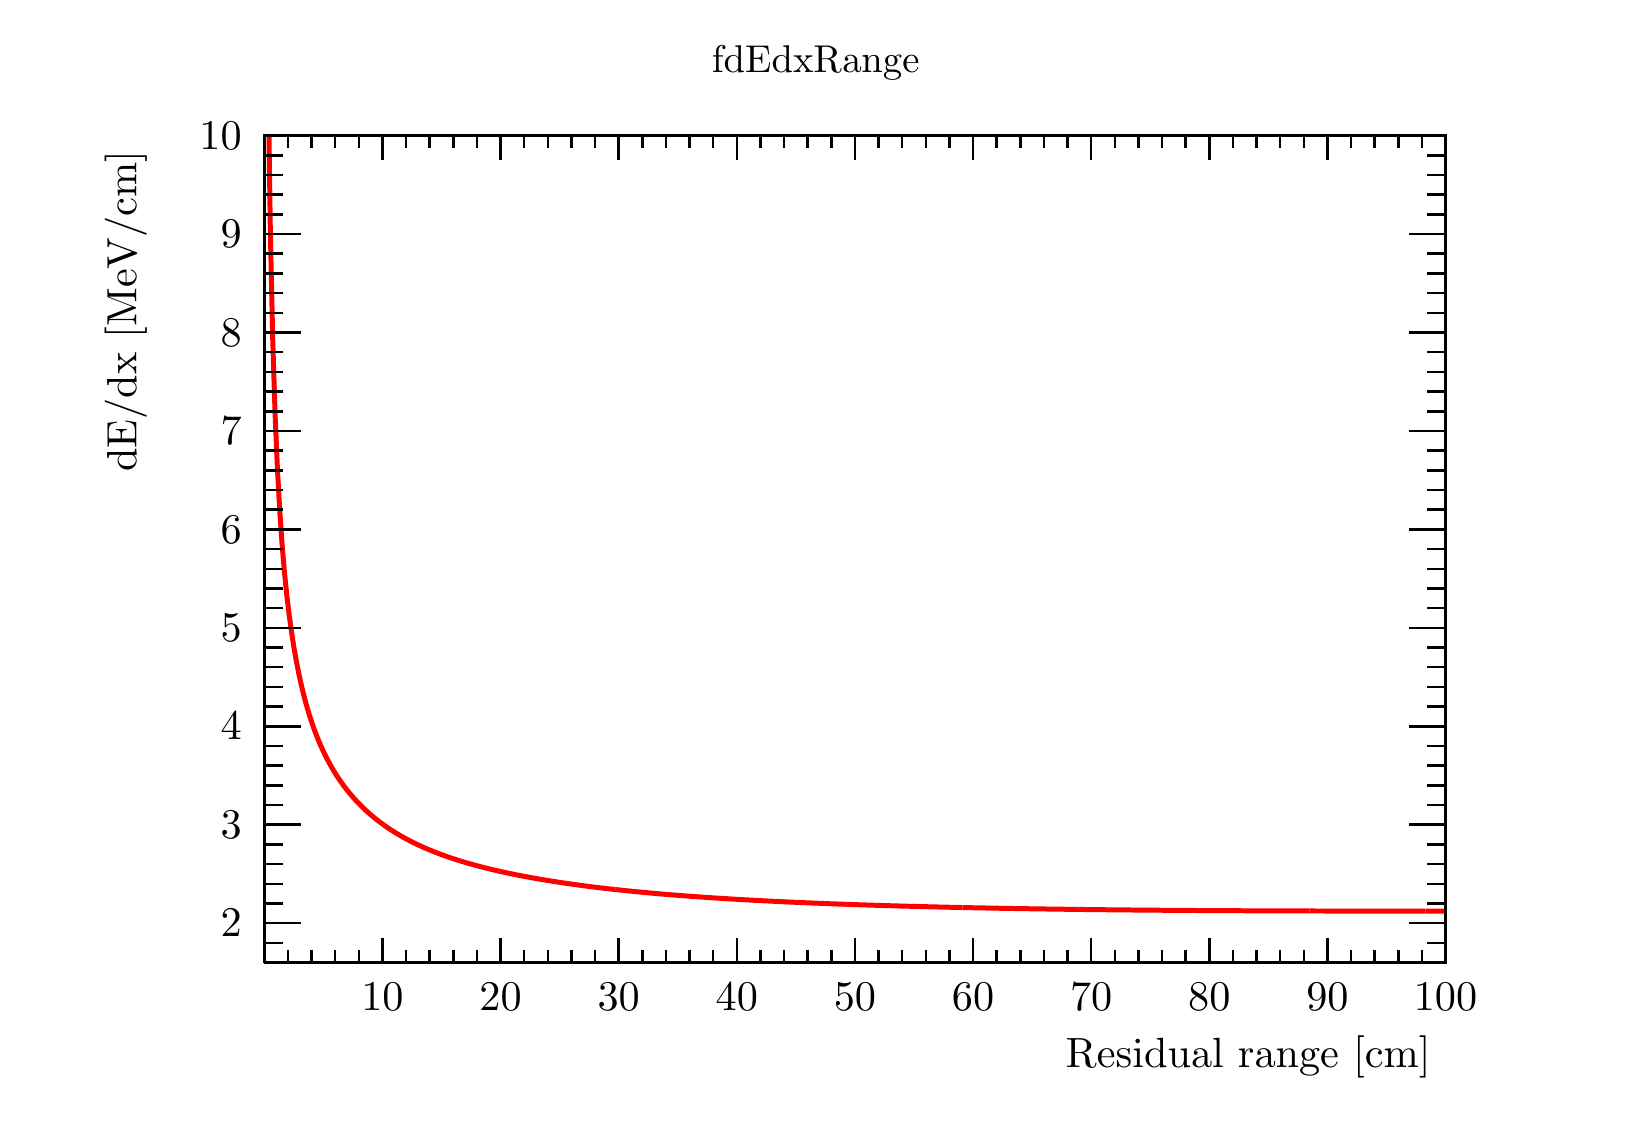
\begin{tikzpicture}
\pgfdeclareplotmark{cross} {
\pgfpathmoveto{\pgfpoint{-0.3\pgfplotmarksize}{\pgfplotmarksize}}
\pgfpathlineto{\pgfpoint{+0.3\pgfplotmarksize}{\pgfplotmarksize}}
\pgfpathlineto{\pgfpoint{+0.3\pgfplotmarksize}{0.3\pgfplotmarksize}}
\pgfpathlineto{\pgfpoint{+1\pgfplotmarksize}{0.3\pgfplotmarksize}}
\pgfpathlineto{\pgfpoint{+1\pgfplotmarksize}{-0.3\pgfplotmarksize}}
\pgfpathlineto{\pgfpoint{+0.3\pgfplotmarksize}{-0.3\pgfplotmarksize}}
\pgfpathlineto{\pgfpoint{+0.3\pgfplotmarksize}{-1.\pgfplotmarksize}}
\pgfpathlineto{\pgfpoint{-0.3\pgfplotmarksize}{-1.\pgfplotmarksize}}
\pgfpathlineto{\pgfpoint{-0.3\pgfplotmarksize}{-0.3\pgfplotmarksize}}
\pgfpathlineto{\pgfpoint{-1.\pgfplotmarksize}{-0.3\pgfplotmarksize}}
\pgfpathlineto{\pgfpoint{-1.\pgfplotmarksize}{0.3\pgfplotmarksize}}
\pgfpathlineto{\pgfpoint{-0.3\pgfplotmarksize}{0.3\pgfplotmarksize}}
\pgfpathclose
\pgfusepathqstroke
}
\pgfdeclareplotmark{cross*} {
\pgfpathmoveto{\pgfpoint{-0.3\pgfplotmarksize}{\pgfplotmarksize}}
\pgfpathlineto{\pgfpoint{+0.3\pgfplotmarksize}{\pgfplotmarksize}}
\pgfpathlineto{\pgfpoint{+0.3\pgfplotmarksize}{0.3\pgfplotmarksize}}
\pgfpathlineto{\pgfpoint{+1\pgfplotmarksize}{0.3\pgfplotmarksize}}
\pgfpathlineto{\pgfpoint{+1\pgfplotmarksize}{-0.3\pgfplotmarksize}}
\pgfpathlineto{\pgfpoint{+0.3\pgfplotmarksize}{-0.3\pgfplotmarksize}}
\pgfpathlineto{\pgfpoint{+0.3\pgfplotmarksize}{-1.\pgfplotmarksize}}
\pgfpathlineto{\pgfpoint{-0.3\pgfplotmarksize}{-1.\pgfplotmarksize}}
\pgfpathlineto{\pgfpoint{-0.3\pgfplotmarksize}{-0.3\pgfplotmarksize}}
\pgfpathlineto{\pgfpoint{-1.\pgfplotmarksize}{-0.3\pgfplotmarksize}}
\pgfpathlineto{\pgfpoint{-1.\pgfplotmarksize}{0.3\pgfplotmarksize}}
\pgfpathlineto{\pgfpoint{-0.3\pgfplotmarksize}{0.3\pgfplotmarksize}}
\pgfpathclose
\pgfusepathqfillstroke
}
\pgfdeclareplotmark{newstar} {
\pgfpathmoveto{\pgfqpoint{0pt}{\pgfplotmarksize}}
\pgfpathlineto{\pgfqpointpolar{44}{0.5\pgfplotmarksize}}
\pgfpathlineto{\pgfqpointpolar{18}{\pgfplotmarksize}}
\pgfpathlineto{\pgfqpointpolar{-20}{0.5\pgfplotmarksize}}
\pgfpathlineto{\pgfqpointpolar{-54}{\pgfplotmarksize}}
\pgfpathlineto{\pgfqpointpolar{-90}{0.5\pgfplotmarksize}}
\pgfpathlineto{\pgfqpointpolar{234}{\pgfplotmarksize}}
\pgfpathlineto{\pgfqpointpolar{198}{0.5\pgfplotmarksize}}
\pgfpathlineto{\pgfqpointpolar{162}{\pgfplotmarksize}}
\pgfpathlineto{\pgfqpointpolar{134}{0.5\pgfplotmarksize}}
\pgfpathclose
\pgfusepathqstroke
}
\pgfdeclareplotmark{newstar*} {
\pgfpathmoveto{\pgfqpoint{0pt}{\pgfplotmarksize}}
\pgfpathlineto{\pgfqpointpolar{44}{0.5\pgfplotmarksize}}
\pgfpathlineto{\pgfqpointpolar{18}{\pgfplotmarksize}}
\pgfpathlineto{\pgfqpointpolar{-20}{0.5\pgfplotmarksize}}
\pgfpathlineto{\pgfqpointpolar{-54}{\pgfplotmarksize}}
\pgfpathlineto{\pgfqpointpolar{-90}{0.5\pgfplotmarksize}}
\pgfpathlineto{\pgfqpointpolar{234}{\pgfplotmarksize}}
\pgfpathlineto{\pgfqpointpolar{198}{0.5\pgfplotmarksize}}
\pgfpathlineto{\pgfqpointpolar{162}{\pgfplotmarksize}}
\pgfpathlineto{\pgfqpointpolar{134}{0.5\pgfplotmarksize}}
\pgfpathclose
\pgfusepathqfillstroke
}
\definecolor{c}{rgb}{1,1,1};
\draw [color=c, fill=c] (0,0) rectangle (20,13.639);
\draw [color=c, fill=c] (3,1.77307) rectangle (18,12.2751);
\definecolor{c}{rgb}{0,0,0};
\draw [c,line width=0.9] (3,1.77307) -- (3,12.2751) -- (18,12.2751) -- (18,1.77307) -- (3,1.77307);
\definecolor{c}{rgb}{1,1,1};
\draw [color=c, fill=c] (3,1.77307) rectangle (18,12.2751);
\definecolor{c}{rgb}{0,0,0};
\draw [c,line width=0.9] (3,1.77307) -- (3,12.2751) -- (18,12.2751) -- (18,1.77307) -- (3,1.77307);
\definecolor{c}{rgb}{1,0,0};
\draw [c,line width=1.8] (3.05761,12.2751) -- (3.075,11.0517);
\draw [c,line width=1.8] (3.075,11.0517) -- (3.105,9.69138) -- (3.135,8.74094) -- (3.165,8.03897) -- (3.195,7.49881) -- (3.225,7.06959) -- (3.255,6.71937) -- (3.285,6.42706) -- (3.315,6.17811) -- (3.345,5.96213) -- (3.375,5.77157) -- (3.405,5.60162)
 -- (3.435,5.44905) -- (3.465,5.31128) -- (3.495,5.18619) -- (3.525,5.07206) -- (3.555,4.96743) -- (3.585,4.87111) -- (3.615,4.78206) -- (3.645,4.69943) -- (3.675,4.62245) -- (3.705,4.5505) -- (3.735,4.48303) -- (3.765,4.4196) -- (3.795,4.35985) --
 (3.825,4.30345) -- (3.855,4.25011) -- (3.885,4.19956) -- (3.915,4.15159) -- (3.945,4.10598) -- (3.975,4.06255) -- (4.005,4.02111) -- (4.035,3.98153) -- (4.065,3.94366) -- (4.095,3.90737) -- (4.125,3.87256) -- (4.155,3.83911) -- (4.185,3.80694) --
 (4.215,3.77598) -- (4.245,3.74616) -- (4.275,3.71743) -- (4.305,3.68973) -- (4.335,3.663) -- (4.365,3.63719) -- (4.395,3.61227) -- (4.425,3.58818) -- (4.455,3.56488) -- (4.485,3.54234) -- (4.515,3.52053);
\draw [c,line width=1.8] (4.515,3.52053) -- (4.545,3.4994) -- (4.575,3.47893) -- (4.605,3.45908) -- (4.635,3.43984) -- (4.665,3.42117) -- (4.695,3.40305) -- (4.725,3.38545) -- (4.755,3.36835) -- (4.785,3.35174) -- (4.815,3.33559) -- (4.845,3.31988)
 -- (4.875,3.3046) -- (4.905,3.28973) -- (4.935,3.27524) -- (4.965,3.26114) -- (4.995,3.2474) -- (5.025,3.23401) -- (5.055,3.22095) -- (5.085,3.20822) -- (5.115,3.1958) -- (5.145,3.18367) -- (5.175,3.17184) -- (5.205,3.16029) -- (5.235,3.149) --
 (5.265,3.13798) -- (5.295,3.12721) -- (5.325,3.11667) -- (5.355,3.10637) -- (5.385,3.0963) -- (5.415,3.08645) -- (5.445,3.07681) -- (5.475,3.06737) -- (5.505,3.05813) -- (5.535,3.04908) -- (5.565,3.04021) -- (5.595,3.03153) -- (5.625,3.02301) --
 (5.655,3.01467) -- (5.685,3.00649) -- (5.715,2.99846) -- (5.745,2.99059) -- (5.775,2.98287) -- (5.805,2.97529) -- (5.835,2.96786) -- (5.865,2.96055) -- (5.895,2.95338) -- (5.925,2.94634) -- (5.955,2.93942) -- (5.985,2.93262);
\draw [c,line width=1.8] (5.985,2.93262) -- (6.015,2.92594) -- (6.045,2.91937) -- (6.075,2.91291) -- (6.105,2.90656) -- (6.135,2.90032) -- (6.165,2.89417) -- (6.195,2.88813) -- (6.225,2.88218) -- (6.255,2.87632) -- (6.285,2.87056) -- (6.315,2.86488)
 -- (6.345,2.8593) -- (6.375,2.85379) -- (6.405,2.84837) -- (6.435,2.84303) -- (6.465,2.83777) -- (6.495,2.83259) -- (6.525,2.82748) -- (6.555,2.82245) -- (6.585,2.81749) -- (6.615,2.81261) -- (6.645,2.8078) -- (6.675,2.80306) -- (6.705,2.79838) --
 (6.735,2.79377) -- (6.765,2.78923) -- (6.795,2.78476) -- (6.825,2.78034) -- (6.855,2.776) -- (6.885,2.77171) -- (6.915,2.76748) -- (6.945,2.76331) -- (6.975,2.7592) -- (7.005,2.75515) -- (7.035,2.75115) -- (7.065,2.74721) -- (7.095,2.74332) --
 (7.125,2.73948) -- (7.155,2.7357) -- (7.185,2.73197) -- (7.215,2.72829) -- (7.245,2.72466) -- (7.275,2.72108) -- (7.305,2.71755) -- (7.335,2.71406) -- (7.365,2.71062) -- (7.395,2.70723) -- (7.425,2.70388) -- (7.455,2.70058);
\draw [c,line width=1.8] (7.455,2.70058) -- (7.485,2.69732) -- (7.515,2.6941) -- (7.545,2.69092) -- (7.575,2.68779) -- (7.605,2.6847) -- (7.635,2.68164) -- (7.665,2.67863) -- (7.695,2.67565) -- (7.725,2.67272) -- (7.755,2.66982) -- (7.785,2.66696) --
 (7.815,2.66413) -- (7.845,2.66134) -- (7.875,2.65858) -- (7.905,2.65586) -- (7.935,2.65318) -- (7.965,2.65053) -- (7.995,2.64791) -- (8.025,2.64532) -- (8.055,2.64276) -- (8.085,2.64024) -- (8.115,2.63775) -- (8.145,2.63528) -- (8.175,2.63285) --
 (8.205,2.63045) -- (8.235,2.62807) -- (8.265,2.62573) -- (8.295,2.62341) -- (8.325,2.62112) -- (8.355,2.61886) -- (8.385,2.61662) -- (8.415,2.61441) -- (8.445,2.61223) -- (8.475,2.61008) -- (8.505,2.60794) -- (8.535,2.60584) -- (8.565,2.60376) --
 (8.595,2.6017) -- (8.625,2.59967) -- (8.655,2.59766) -- (8.685,2.59567) -- (8.715,2.59371) -- (8.745,2.59177) -- (8.775,2.58985) -- (8.805,2.58795) -- (8.835,2.58608) -- (8.865,2.58422) -- (8.895,2.58239) -- (8.925,2.58058);
\draw [c,line width=1.8] (8.925,2.58058) -- (8.955,2.57879) -- (8.985,2.57702) -- (9.015,2.57527) -- (9.045,2.57354) -- (9.075,2.57182) -- (9.105,2.57013) -- (9.135,2.56846) -- (9.165,2.5668) -- (9.195,2.56517) -- (9.225,2.56355) -- (9.255,2.56195)
 -- (9.285,2.56036) -- (9.315,2.5588) -- (9.345,2.55725) -- (9.375,2.55572) -- (9.405,2.5542) -- (9.435,2.5527) -- (9.465,2.55122) -- (9.495,2.54975) -- (9.525,2.5483) -- (9.555,2.54687) -- (9.585,2.54545) -- (9.615,2.54405) -- (9.645,2.54266) --
 (9.675,2.54129) -- (9.705,2.53993) -- (9.735,2.53858) -- (9.765,2.53725) -- (9.795,2.53594) -- (9.825,2.53463) -- (9.855,2.53335) -- (9.885,2.53207) -- (9.915,2.53081) -- (9.945,2.52956) -- (9.975,2.52833) -- (10.005,2.52711) -- (10.035,2.5259) --
 (10.065,2.5247) -- (10.095,2.52352) -- (10.125,2.52235) -- (10.155,2.52119) -- (10.185,2.52005) -- (10.215,2.51891) -- (10.245,2.51779) -- (10.275,2.51668) -- (10.305,2.51558) -- (10.335,2.51449) -- (10.365,2.51342) -- (10.395,2.51235);
\draw [c,line width=1.8] (10.395,2.51235) -- (10.425,2.5113) -- (10.455,2.51025) -- (10.485,2.50922) -- (10.515,2.5082) -- (10.545,2.50719) -- (10.575,2.50619) -- (10.605,2.5052) -- (10.635,2.50422) -- (10.665,2.50325) -- (10.695,2.50229) --
 (10.725,2.50134) -- (10.755,2.5004) -- (10.785,2.49947) -- (10.815,2.49855) -- (10.845,2.49764) -- (10.875,2.49674) -- (10.905,2.49584) -- (10.935,2.49496) -- (10.965,2.49409) -- (10.995,2.49322) -- (11.025,2.49237) -- (11.055,2.49152) --
 (11.085,2.49068) -- (11.115,2.48986) -- (11.145,2.48903) -- (11.175,2.48822) -- (11.205,2.48742) -- (11.235,2.48662) -- (11.265,2.48584) -- (11.295,2.48506) -- (11.325,2.48429) -- (11.355,2.48353) -- (11.385,2.48277) -- (11.415,2.48203) --
 (11.445,2.48129) -- (11.475,2.48056) -- (11.505,2.47983) -- (11.535,2.47912) -- (11.565,2.47841) -- (11.595,2.47771) -- (11.625,2.47701) -- (11.655,2.47633) -- (11.685,2.47565) -- (11.715,2.47498) -- (11.745,2.47431) -- (11.775,2.47366) --
 (11.805,2.473) -- (11.835,2.47236) -- (11.865,2.47172);
\draw [c,line width=1.8] (11.865,2.47172) -- (11.895,2.47109) -- (11.925,2.47047) -- (11.955,2.46985) -- (11.985,2.46924) -- (12.015,2.46864) -- (12.045,2.46804) -- (12.075,2.46745) -- (12.105,2.46687) -- (12.135,2.46629) -- (12.165,2.46572) --
 (12.195,2.46515) -- (12.225,2.46459) -- (12.255,2.46404) -- (12.285,2.46349) -- (12.315,2.46295) -- (12.345,2.46241) -- (12.375,2.46188) -- (12.405,2.46135) -- (12.435,2.46084) -- (12.465,2.46032) -- (12.495,2.45982) -- (12.525,2.45931) --
 (12.555,2.45882) -- (12.585,2.45833) -- (12.615,2.45784) -- (12.645,2.45736) -- (12.675,2.45689) -- (12.705,2.45642) -- (12.735,2.45595) -- (12.765,2.45549) -- (12.795,2.45504) -- (12.825,2.45459) -- (12.855,2.45414) -- (12.885,2.45371) --
 (12.915,2.45327) -- (12.945,2.45284) -- (12.975,2.45242) -- (13.005,2.452) -- (13.035,2.45158) -- (13.065,2.45117) -- (13.095,2.45077) -- (13.125,2.45037) -- (13.155,2.44997) -- (13.185,2.44958) -- (13.215,2.44919) -- (13.245,2.44881) --
 (13.275,2.44843) -- (13.305,2.44806) -- (13.335,2.44769);
\draw [c,line width=1.8] (13.335,2.44769) -- (13.365,2.44733) -- (13.395,2.44697) -- (13.425,2.44661) -- (13.455,2.44626) -- (13.485,2.44591) -- (13.515,2.44557) -- (13.545,2.44523) -- (13.575,2.44489) -- (13.605,2.44456) -- (13.635,2.44423) --
 (13.665,2.44391) -- (13.695,2.44359) -- (13.725,2.44328) -- (13.755,2.44297) -- (13.785,2.44266) -- (13.815,2.44235) -- (13.845,2.44205) -- (13.875,2.44176) -- (13.905,2.44147) -- (13.935,2.44118) -- (13.965,2.44089) -- (13.995,2.44061) --
 (14.025,2.44033) -- (14.055,2.44006) -- (14.085,2.43979) -- (14.115,2.43952) -- (14.145,2.43926) -- (14.175,2.439) -- (14.205,2.43874) -- (14.235,2.43849) -- (14.265,2.43824) -- (14.295,2.43799) -- (14.325,2.43775) -- (14.355,2.43751) --
 (14.385,2.43727) -- (14.415,2.43704) -- (14.445,2.43681) -- (14.475,2.43658) -- (14.505,2.43636) -- (14.535,2.43614) -- (14.565,2.43592) -- (14.595,2.43571) -- (14.625,2.4355) -- (14.655,2.43529) -- (14.685,2.43508) -- (14.715,2.43488) --
 (14.745,2.43468) -- (14.775,2.43449) -- (14.805,2.43429);
\draw [c,line width=1.8] (14.805,2.43429) -- (14.835,2.4341) -- (14.865,2.43392) -- (14.895,2.43373) -- (14.925,2.43355) -- (14.955,2.43337) -- (14.985,2.4332) -- (15.015,2.43302) -- (15.045,2.43285) -- (15.075,2.43269) -- (15.105,2.43252) --
 (15.135,2.43236) -- (15.165,2.4322) -- (15.195,2.43204) -- (15.225,2.43189) -- (15.255,2.43174) -- (15.285,2.43159) -- (15.315,2.43144) -- (15.345,2.4313) -- (15.375,2.43116) -- (15.405,2.43102) -- (15.435,2.43088) -- (15.465,2.43075) --
 (15.495,2.43062) -- (15.525,2.43049) -- (15.555,2.43037) -- (15.585,2.43024) -- (15.615,2.43012) -- (15.645,2.43) -- (15.675,2.42989) -- (15.705,2.42977) -- (15.735,2.42966) -- (15.765,2.42955) -- (15.795,2.42944) -- (15.825,2.42934) --
 (15.855,2.42924) -- (15.885,2.42914) -- (15.915,2.42904) -- (15.945,2.42894) -- (15.975,2.42885) -- (16.005,2.42876) -- (16.035,2.42867) -- (16.065,2.42858) -- (16.095,2.4285) -- (16.125,2.42841) -- (16.155,2.42833) -- (16.185,2.42825) --
 (16.215,2.42818) -- (16.245,2.4281) -- (16.275,2.42803);
\draw [c,line width=1.8] (16.275,2.42803) -- (16.305,2.42796) -- (16.335,2.42789) -- (16.365,2.42782) -- (16.395,2.42776) -- (16.425,2.4277) -- (16.455,2.42764) -- (16.485,2.42758) -- (16.515,2.42752) -- (16.545,2.42747) -- (16.575,2.42741) --
 (16.605,2.42736) -- (16.635,2.42731) -- (16.665,2.42727) -- (16.695,2.42722) -- (16.725,2.42718) -- (16.755,2.42714) -- (16.785,2.4271) -- (16.815,2.42706) -- (16.845,2.42702) -- (16.875,2.42699) -- (16.905,2.42696) -- (16.935,2.42693) --
 (16.965,2.4269) -- (16.995,2.42687) -- (17.025,2.42684) -- (17.055,2.42682) -- (17.085,2.4268) -- (17.115,2.42678) -- (17.145,2.42676) -- (17.175,2.42674) -- (17.205,2.42673) -- (17.235,2.42671) -- (17.265,2.4267) -- (17.295,2.42669) --
 (17.325,2.42668) -- (17.355,2.42667) -- (17.385,2.42667) -- (17.415,2.42666) -- (17.445,2.42666) -- (17.475,2.42666) -- (17.505,2.42666) -- (17.535,2.42666) -- (17.565,2.42666) -- (17.595,2.42667) -- (17.625,2.42668) -- (17.655,2.42668) --
 (17.685,2.42669) -- (17.715,2.4267) -- (17.745,2.42672);
\draw [c,line width=1.8] (17.745,2.42672) -- (17.775,2.42673) -- (17.805,2.42674) -- (17.835,2.42676) -- (17.865,2.42678) -- (17.895,2.4268) -- (17.925,2.42682) -- (17.955,2.42684) -- (17.985,2.42686);
\definecolor{c}{rgb}{0,0,0};
\draw [c,line width=0.9] (3,1.77307) -- (18,1.77307);
\draw [c,line width=0.9] (4.49865,2.07994) -- (4.49865,1.77307);
\draw [c,line width=0.9] (4.79868,1.9265) -- (4.79868,1.77307);
\draw [c,line width=0.9] (5.09871,1.9265) -- (5.09871,1.77307);
\draw [c,line width=0.9] (5.39874,1.9265) -- (5.39874,1.77307);
\draw [c,line width=0.9] (5.69877,1.9265) -- (5.69877,1.77307);
\draw [c,line width=0.9] (5.9988,2.07994) -- (5.9988,1.77307);
\draw [c,line width=0.9] (6.29883,1.9265) -- (6.29883,1.77307);
\draw [c,line width=0.9] (6.59886,1.9265) -- (6.59886,1.77307);
\draw [c,line width=0.9] (6.89889,1.9265) -- (6.89889,1.77307);
\draw [c,line width=0.9] (7.19892,1.9265) -- (7.19892,1.77307);
\draw [c,line width=0.9] (7.49895,2.07994) -- (7.49895,1.77307);
\draw [c,line width=0.9] (7.79898,1.9265) -- (7.79898,1.77307);
\draw [c,line width=0.9] (8.09901,1.9265) -- (8.09901,1.77307);
\draw [c,line width=0.9] (8.39904,1.9265) -- (8.39904,1.77307);
\draw [c,line width=0.9] (8.69907,1.9265) -- (8.69907,1.77307);
\draw [c,line width=0.9] (8.9991,2.07994) -- (8.9991,1.77307);
\draw [c,line width=0.9] (9.29913,1.9265) -- (9.29913,1.77307);
\draw [c,line width=0.9] (9.59916,1.9265) -- (9.59916,1.77307);
\draw [c,line width=0.9] (9.89919,1.9265) -- (9.89919,1.77307);
\draw [c,line width=0.9] (10.1992,1.9265) -- (10.1992,1.77307);
\draw [c,line width=0.9] (10.4993,2.07994) -- (10.4993,1.77307);
\draw [c,line width=0.9] (10.7993,1.9265) -- (10.7993,1.77307);
\draw [c,line width=0.9] (11.0993,1.9265) -- (11.0993,1.77307);
\draw [c,line width=0.9] (11.3993,1.9265) -- (11.3993,1.77307);
\draw [c,line width=0.9] (11.6994,1.9265) -- (11.6994,1.77307);
\draw [c,line width=0.9] (11.9994,2.07994) -- (11.9994,1.77307);
\draw [c,line width=0.9] (12.2994,1.9265) -- (12.2994,1.77307);
\draw [c,line width=0.9] (12.5995,1.9265) -- (12.5995,1.77307);
\draw [c,line width=0.9] (12.8995,1.9265) -- (12.8995,1.77307);
\draw [c,line width=0.9] (13.1995,1.9265) -- (13.1995,1.77307);
\draw [c,line width=0.9] (13.4995,2.07994) -- (13.4995,1.77307);
\draw [c,line width=0.9] (13.7996,1.9265) -- (13.7996,1.77307);
\draw [c,line width=0.9] (14.0996,1.9265) -- (14.0996,1.77307);
\draw [c,line width=0.9] (14.3996,1.9265) -- (14.3996,1.77307);
\draw [c,line width=0.9] (14.6997,1.9265) -- (14.6997,1.77307);
\draw [c,line width=0.9] (14.9997,2.07994) -- (14.9997,1.77307);
\draw [c,line width=0.9] (15.2997,1.9265) -- (15.2997,1.77307);
\draw [c,line width=0.9] (15.5998,1.9265) -- (15.5998,1.77307);
\draw [c,line width=0.9] (15.8998,1.9265) -- (15.8998,1.77307);
\draw [c,line width=0.9] (16.1998,1.9265) -- (16.1998,1.77307);
\draw [c,line width=0.9] (16.4998,2.07994) -- (16.4998,1.77307);
\draw [c,line width=0.9] (16.7999,1.9265) -- (16.7999,1.77307);
\draw [c,line width=0.9] (17.0999,1.9265) -- (17.0999,1.77307);
\draw [c,line width=0.9] (17.3999,1.9265) -- (17.3999,1.77307);
\draw [c,line width=0.9] (17.7,1.9265) -- (17.7,1.77307);
\draw [c,line width=0.9] (18,2.07994) -- (18,1.77307);
\draw [c,line width=0.9] (4.49865,2.07994) -- (4.49865,1.77307);
\draw [c,line width=0.9] (4.19862,1.9265) -- (4.19862,1.77307);
\draw [c,line width=0.9] (3.89859,1.9265) -- (3.89859,1.77307);
\draw [c,line width=0.9] (3.59856,1.9265) -- (3.59856,1.77307);
\draw [c,line width=0.9] (3.29853,1.9265) -- (3.29853,1.77307);
\draw [anchor=base] (4.49865,1.15931) node[scale=1.52731, color=c, rotate=0]{10};
\draw [anchor=base] (5.9988,1.15931) node[scale=1.52731, color=c, rotate=0]{20};
\draw [anchor=base] (7.49895,1.15931) node[scale=1.52731, color=c, rotate=0]{30};
\draw [anchor=base] (8.9991,1.15931) node[scale=1.52731, color=c, rotate=0]{40};
\draw [anchor=base] (10.4993,1.15931) node[scale=1.52731, color=c, rotate=0]{50};
\draw [anchor=base] (11.9994,1.15931) node[scale=1.52731, color=c, rotate=0]{60};
\draw [anchor=base] (13.4995,1.15931) node[scale=1.52731, color=c, rotate=0]{70};
\draw [anchor=base] (14.9997,1.15931) node[scale=1.52731, color=c, rotate=0]{80};
\draw [anchor=base] (16.4998,1.15931) node[scale=1.52731, color=c, rotate=0]{90};
\draw [anchor=base] (18,1.15931) node[scale=1.52731, color=c, rotate=0]{100};
\draw [anchor= east] (18,0.572837) node[scale=1.52731, color=c, rotate=0]{Residual range [cm]};
\draw [c,line width=0.9] (3,12.2751) -- (18,12.2751);
\draw [c,line width=0.9] (4.49865,11.9682) -- (4.49865,12.2751);
\draw [c,line width=0.9] (4.79868,12.1216) -- (4.79868,12.2751);
\draw [c,line width=0.9] (5.09871,12.1216) -- (5.09871,12.2751);
\draw [c,line width=0.9] (5.39874,12.1216) -- (5.39874,12.2751);
\draw [c,line width=0.9] (5.69877,12.1216) -- (5.69877,12.2751);
\draw [c,line width=0.9] (5.9988,11.9682) -- (5.9988,12.2751);
\draw [c,line width=0.9] (6.29883,12.1216) -- (6.29883,12.2751);
\draw [c,line width=0.9] (6.59886,12.1216) -- (6.59886,12.2751);
\draw [c,line width=0.9] (6.89889,12.1216) -- (6.89889,12.2751);
\draw [c,line width=0.9] (7.19892,12.1216) -- (7.19892,12.2751);
\draw [c,line width=0.9] (7.49895,11.9682) -- (7.49895,12.2751);
\draw [c,line width=0.9] (7.79898,12.1216) -- (7.79898,12.2751);
\draw [c,line width=0.9] (8.09901,12.1216) -- (8.09901,12.2751);
\draw [c,line width=0.9] (8.39904,12.1216) -- (8.39904,12.2751);
\draw [c,line width=0.9] (8.69907,12.1216) -- (8.69907,12.2751);
\draw [c,line width=0.9] (8.9991,11.9682) -- (8.9991,12.2751);
\draw [c,line width=0.9] (9.29913,12.1216) -- (9.29913,12.2751);
\draw [c,line width=0.9] (9.59916,12.1216) -- (9.59916,12.2751);
\draw [c,line width=0.9] (9.89919,12.1216) -- (9.89919,12.2751);
\draw [c,line width=0.9] (10.1992,12.1216) -- (10.1992,12.2751);
\draw [c,line width=0.9] (10.4993,11.9682) -- (10.4993,12.2751);
\draw [c,line width=0.9] (10.7993,12.1216) -- (10.7993,12.2751);
\draw [c,line width=0.9] (11.0993,12.1216) -- (11.0993,12.2751);
\draw [c,line width=0.9] (11.3993,12.1216) -- (11.3993,12.2751);
\draw [c,line width=0.9] (11.6994,12.1216) -- (11.6994,12.2751);
\draw [c,line width=0.9] (11.9994,11.9682) -- (11.9994,12.2751);
\draw [c,line width=0.9] (12.2994,12.1216) -- (12.2994,12.2751);
\draw [c,line width=0.9] (12.5995,12.1216) -- (12.5995,12.2751);
\draw [c,line width=0.9] (12.8995,12.1216) -- (12.8995,12.2751);
\draw [c,line width=0.9] (13.1995,12.1216) -- (13.1995,12.2751);
\draw [c,line width=0.9] (13.4995,11.9682) -- (13.4995,12.2751);
\draw [c,line width=0.9] (13.7996,12.1216) -- (13.7996,12.2751);
\draw [c,line width=0.9] (14.0996,12.1216) -- (14.0996,12.2751);
\draw [c,line width=0.9] (14.3996,12.1216) -- (14.3996,12.2751);
\draw [c,line width=0.9] (14.6997,12.1216) -- (14.6997,12.2751);
\draw [c,line width=0.9] (14.9997,11.9682) -- (14.9997,12.2751);
\draw [c,line width=0.9] (15.2997,12.1216) -- (15.2997,12.2751);
\draw [c,line width=0.9] (15.5998,12.1216) -- (15.5998,12.2751);
\draw [c,line width=0.9] (15.8998,12.1216) -- (15.8998,12.2751);
\draw [c,line width=0.9] (16.1998,12.1216) -- (16.1998,12.2751);
\draw [c,line width=0.9] (16.4998,11.9682) -- (16.4998,12.2751);
\draw [c,line width=0.9] (16.7999,12.1216) -- (16.7999,12.2751);
\draw [c,line width=0.9] (17.0999,12.1216) -- (17.0999,12.2751);
\draw [c,line width=0.9] (17.3999,12.1216) -- (17.3999,12.2751);
\draw [c,line width=0.9] (17.7,12.1216) -- (17.7,12.2751);
\draw [c,line width=0.9] (18,11.9682) -- (18,12.2751);
\draw [c,line width=0.9] (4.49865,11.9682) -- (4.49865,12.2751);
\draw [c,line width=0.9] (4.19862,12.1216) -- (4.19862,12.2751);
\draw [c,line width=0.9] (3.89859,12.1216) -- (3.89859,12.2751);
\draw [c,line width=0.9] (3.59856,12.1216) -- (3.59856,12.2751);
\draw [c,line width=0.9] (3.29853,12.1216) -- (3.29853,12.2751);
\draw [c,line width=0.9] (3,1.77307) -- (3,12.2751);
\draw [c,line width=0.9] (3.462,2.27316) -- (3,2.27316);
\draw [c,line width=0.9] (3.231,2.52321) -- (3,2.52321);
\draw [c,line width=0.9] (3.231,2.77326) -- (3,2.77326);
\draw [c,line width=0.9] (3.231,3.0233) -- (3,3.0233);
\draw [c,line width=0.9] (3.231,3.27335) -- (3,3.27335);
\draw [c,line width=0.9] (3.462,3.5234) -- (3,3.5234);
\draw [c,line width=0.9] (3.231,3.77345) -- (3,3.77345);
\draw [c,line width=0.9] (3.231,4.0235) -- (3,4.0235);
\draw [c,line width=0.9] (3.231,4.27354) -- (3,4.27354);
\draw [c,line width=0.9] (3.231,4.52359) -- (3,4.52359);
\draw [c,line width=0.9] (3.462,4.77364) -- (3,4.77364);
\draw [c,line width=0.9] (3.231,5.02369) -- (3,5.02369);
\draw [c,line width=0.9] (3.231,5.27373) -- (3,5.27373);
\draw [c,line width=0.9] (3.231,5.52378) -- (3,5.52378);
\draw [c,line width=0.9] (3.231,5.77383) -- (3,5.77383);
\draw [c,line width=0.9] (3.462,6.02388) -- (3,6.02388);
\draw [c,line width=0.9] (3.231,6.27393) -- (3,6.27393);
\draw [c,line width=0.9] (3.231,6.52397) -- (3,6.52397);
\draw [c,line width=0.9] (3.231,6.77402) -- (3,6.77402);
\draw [c,line width=0.9] (3.231,7.02407) -- (3,7.02407);
\draw [c,line width=0.9] (3.462,7.27412) -- (3,7.27412);
\draw [c,line width=0.9] (3.231,7.52416) -- (3,7.52416);
\draw [c,line width=0.9] (3.231,7.77421) -- (3,7.77421);
\draw [c,line width=0.9] (3.231,8.02426) -- (3,8.02426);
\draw [c,line width=0.9] (3.231,8.27431) -- (3,8.27431);
\draw [c,line width=0.9] (3.462,8.52435) -- (3,8.52435);
\draw [c,line width=0.9] (3.231,8.7744) -- (3,8.7744);
\draw [c,line width=0.9] (3.231,9.02445) -- (3,9.02445);
\draw [c,line width=0.9] (3.231,9.2745) -- (3,9.2745);
\draw [c,line width=0.9] (3.231,9.52455) -- (3,9.52455);
\draw [c,line width=0.9] (3.462,9.77459) -- (3,9.77459);
\draw [c,line width=0.9] (3.231,10.0246) -- (3,10.0246);
\draw [c,line width=0.9] (3.231,10.2747) -- (3,10.2747);
\draw [c,line width=0.9] (3.231,10.5247) -- (3,10.5247);
\draw [c,line width=0.9] (3.231,10.7748) -- (3,10.7748);
\draw [c,line width=0.9] (3.462,11.0248) -- (3,11.0248);
\draw [c,line width=0.9] (3.231,11.2749) -- (3,11.2749);
\draw [c,line width=0.9] (3.231,11.5249) -- (3,11.5249);
\draw [c,line width=0.9] (3.231,11.775) -- (3,11.775);
\draw [c,line width=0.9] (3.231,12.025) -- (3,12.025);
\draw [c,line width=0.9] (3.462,12.2751) -- (3,12.2751);
\draw [c,line width=0.9] (3.462,2.27316) -- (3,2.27316);
\draw [c,line width=0.9] (3.231,2.02311) -- (3,2.02311);
\draw [c,line width=0.9] (3.231,1.77307) -- (3,1.77307);
\draw [anchor= east] (2.9,2.27316) node[scale=1.52731, color=c, rotate=0]{2};
\draw [anchor= east] (2.9,3.5234) node[scale=1.52731, color=c, rotate=0]{3};
\draw [anchor= east] (2.9,4.77364) node[scale=1.52731, color=c, rotate=0]{4};
\draw [anchor= east] (2.9,6.02388) node[scale=1.52731, color=c, rotate=0]{5};
\draw [anchor= east] (2.9,7.27412) node[scale=1.52731, color=c, rotate=0]{6};
\draw [anchor= east] (2.9,8.52435) node[scale=1.52731, color=c, rotate=0]{7};
\draw [anchor= east] (2.9,9.77459) node[scale=1.52731, color=c, rotate=0]{8};
\draw [anchor= east] (2.9,11.0248) node[scale=1.52731, color=c, rotate=0]{9};
\draw [anchor= east] (2.9,12.2751) node[scale=1.52731, color=c, rotate=0]{10};
\draw [anchor= east] (1.24,12.2751) node[scale=1.52731, color=c, rotate=90]{dE/dx [MeV/cm]};
\draw [c,line width=0.9] (18,1.77307) -- (18,12.2751);
\draw [c,line width=0.9] (17.538,2.27316) -- (18,2.27316);
\draw [c,line width=0.9] (17.769,2.52321) -- (18,2.52321);
\draw [c,line width=0.9] (17.769,2.77326) -- (18,2.77326);
\draw [c,line width=0.9] (17.769,3.0233) -- (18,3.0233);
\draw [c,line width=0.9] (17.769,3.27335) -- (18,3.27335);
\draw [c,line width=0.9] (17.538,3.5234) -- (18,3.5234);
\draw [c,line width=0.9] (17.769,3.77345) -- (18,3.77345);
\draw [c,line width=0.9] (17.769,4.0235) -- (18,4.0235);
\draw [c,line width=0.9] (17.769,4.27354) -- (18,4.27354);
\draw [c,line width=0.9] (17.769,4.52359) -- (18,4.52359);
\draw [c,line width=0.9] (17.538,4.77364) -- (18,4.77364);
\draw [c,line width=0.9] (17.769,5.02369) -- (18,5.02369);
\draw [c,line width=0.9] (17.769,5.27373) -- (18,5.27373);
\draw [c,line width=0.9] (17.769,5.52378) -- (18,5.52378);
\draw [c,line width=0.9] (17.769,5.77383) -- (18,5.77383);
\draw [c,line width=0.9] (17.538,6.02388) -- (18,6.02388);
\draw [c,line width=0.9] (17.769,6.27393) -- (18,6.27393);
\draw [c,line width=0.9] (17.769,6.52397) -- (18,6.52397);
\draw [c,line width=0.9] (17.769,6.77402) -- (18,6.77402);
\draw [c,line width=0.9] (17.769,7.02407) -- (18,7.02407);
\draw [c,line width=0.9] (17.538,7.27412) -- (18,7.27412);
\draw [c,line width=0.9] (17.769,7.52416) -- (18,7.52416);
\draw [c,line width=0.9] (17.769,7.77421) -- (18,7.77421);
\draw [c,line width=0.9] (17.769,8.02426) -- (18,8.02426);
\draw [c,line width=0.9] (17.769,8.27431) -- (18,8.27431);
\draw [c,line width=0.9] (17.538,8.52435) -- (18,8.52435);
\draw [c,line width=0.9] (17.769,8.7744) -- (18,8.7744);
\draw [c,line width=0.9] (17.769,9.02445) -- (18,9.02445);
\draw [c,line width=0.9] (17.769,9.2745) -- (18,9.2745);
\draw [c,line width=0.9] (17.769,9.52455) -- (18,9.52455);
\draw [c,line width=0.9] (17.538,9.77459) -- (18,9.77459);
\draw [c,line width=0.9] (17.769,10.0246) -- (18,10.0246);
\draw [c,line width=0.9] (17.769,10.2747) -- (18,10.2747);
\draw [c,line width=0.9] (17.769,10.5247) -- (18,10.5247);
\draw [c,line width=0.9] (17.769,10.7748) -- (18,10.7748);
\draw [c,line width=0.9] (17.538,11.0248) -- (18,11.0248);
\draw [c,line width=0.9] (17.769,11.2749) -- (18,11.2749);
\draw [c,line width=0.9] (17.769,11.5249) -- (18,11.5249);
\draw [c,line width=0.9] (17.769,11.775) -- (18,11.775);
\draw [c,line width=0.9] (17.769,12.025) -- (18,12.025);
\draw [c,line width=0.9] (17.538,12.2751) -- (18,12.2751);
\draw [c,line width=0.9] (17.538,2.27316) -- (18,2.27316);
\draw [c,line width=0.9] (17.769,2.02311) -- (18,2.02311);
\draw [c,line width=0.9] (17.769,1.77307) -- (18,1.77307);
\definecolor{c}{rgb}{1,1,1};
\draw [color=c, fill=c] (2,12.8206) rectangle (18,13.5708);
\definecolor{c}{rgb}{0,0,0};
\draw (10,13.1957) node[scale=1.40004, color=c, rotate=0]{fdEdxRange};
\end{tikzpicture}

		\end{adjustbox}
	\end{minipage}
	\hfill
	\begin{minipage}[t]{.5\linewidth}
		\begin{adjustbox}{max totalsize=\linewidth, center}
			\begin{tikzpicture}
\pgfdeclareplotmark{cross} {
\pgfpathmoveto{\pgfpoint{-0.3\pgfplotmarksize}{\pgfplotmarksize}}
\pgfpathlineto{\pgfpoint{+0.3\pgfplotmarksize}{\pgfplotmarksize}}
\pgfpathlineto{\pgfpoint{+0.3\pgfplotmarksize}{0.3\pgfplotmarksize}}
\pgfpathlineto{\pgfpoint{+1\pgfplotmarksize}{0.3\pgfplotmarksize}}
\pgfpathlineto{\pgfpoint{+1\pgfplotmarksize}{-0.3\pgfplotmarksize}}
\pgfpathlineto{\pgfpoint{+0.3\pgfplotmarksize}{-0.3\pgfplotmarksize}}
\pgfpathlineto{\pgfpoint{+0.3\pgfplotmarksize}{-1.\pgfplotmarksize}}
\pgfpathlineto{\pgfpoint{-0.3\pgfplotmarksize}{-1.\pgfplotmarksize}}
\pgfpathlineto{\pgfpoint{-0.3\pgfplotmarksize}{-0.3\pgfplotmarksize}}
\pgfpathlineto{\pgfpoint{-1.\pgfplotmarksize}{-0.3\pgfplotmarksize}}
\pgfpathlineto{\pgfpoint{-1.\pgfplotmarksize}{0.3\pgfplotmarksize}}
\pgfpathlineto{\pgfpoint{-0.3\pgfplotmarksize}{0.3\pgfplotmarksize}}
\pgfpathclose
\pgfusepathqstroke
}
\pgfdeclareplotmark{cross*} {
\pgfpathmoveto{\pgfpoint{-0.3\pgfplotmarksize}{\pgfplotmarksize}}
\pgfpathlineto{\pgfpoint{+0.3\pgfplotmarksize}{\pgfplotmarksize}}
\pgfpathlineto{\pgfpoint{+0.3\pgfplotmarksize}{0.3\pgfplotmarksize}}
\pgfpathlineto{\pgfpoint{+1\pgfplotmarksize}{0.3\pgfplotmarksize}}
\pgfpathlineto{\pgfpoint{+1\pgfplotmarksize}{-0.3\pgfplotmarksize}}
\pgfpathlineto{\pgfpoint{+0.3\pgfplotmarksize}{-0.3\pgfplotmarksize}}
\pgfpathlineto{\pgfpoint{+0.3\pgfplotmarksize}{-1.\pgfplotmarksize}}
\pgfpathlineto{\pgfpoint{-0.3\pgfplotmarksize}{-1.\pgfplotmarksize}}
\pgfpathlineto{\pgfpoint{-0.3\pgfplotmarksize}{-0.3\pgfplotmarksize}}
\pgfpathlineto{\pgfpoint{-1.\pgfplotmarksize}{-0.3\pgfplotmarksize}}
\pgfpathlineto{\pgfpoint{-1.\pgfplotmarksize}{0.3\pgfplotmarksize}}
\pgfpathlineto{\pgfpoint{-0.3\pgfplotmarksize}{0.3\pgfplotmarksize}}
\pgfpathclose
\pgfusepathqfillstroke
}
\pgfdeclareplotmark{newstar} {
\pgfpathmoveto{\pgfqpoint{0pt}{\pgfplotmarksize}}
\pgfpathlineto{\pgfqpointpolar{44}{0.5\pgfplotmarksize}}
\pgfpathlineto{\pgfqpointpolar{18}{\pgfplotmarksize}}
\pgfpathlineto{\pgfqpointpolar{-20}{0.5\pgfplotmarksize}}
\pgfpathlineto{\pgfqpointpolar{-54}{\pgfplotmarksize}}
\pgfpathlineto{\pgfqpointpolar{-90}{0.5\pgfplotmarksize}}
\pgfpathlineto{\pgfqpointpolar{234}{\pgfplotmarksize}}
\pgfpathlineto{\pgfqpointpolar{198}{0.5\pgfplotmarksize}}
\pgfpathlineto{\pgfqpointpolar{162}{\pgfplotmarksize}}
\pgfpathlineto{\pgfqpointpolar{134}{0.5\pgfplotmarksize}}
\pgfpathclose
\pgfusepathqstroke
}
\pgfdeclareplotmark{newstar*} {
\pgfpathmoveto{\pgfqpoint{0pt}{\pgfplotmarksize}}
\pgfpathlineto{\pgfqpointpolar{44}{0.5\pgfplotmarksize}}
\pgfpathlineto{\pgfqpointpolar{18}{\pgfplotmarksize}}
\pgfpathlineto{\pgfqpointpolar{-20}{0.5\pgfplotmarksize}}
\pgfpathlineto{\pgfqpointpolar{-54}{\pgfplotmarksize}}
\pgfpathlineto{\pgfqpointpolar{-90}{0.5\pgfplotmarksize}}
\pgfpathlineto{\pgfqpointpolar{234}{\pgfplotmarksize}}
\pgfpathlineto{\pgfqpointpolar{198}{0.5\pgfplotmarksize}}
\pgfpathlineto{\pgfqpointpolar{162}{\pgfplotmarksize}}
\pgfpathlineto{\pgfqpointpolar{134}{0.5\pgfplotmarksize}}
\pgfpathclose
\pgfusepathqfillstroke
}
\definecolor{c}{rgb}{1,1,1};
\draw [color=c, fill=c] (0,0) rectangle (20,13.639);
\draw [color=c, fill=c] (3,1.77307) rectangle (18,12.2751);
\definecolor{c}{rgb}{0,0,0};
\draw [c,line width=0.9] (3,1.77307) -- (3,12.2751) -- (18,12.2751) -- (18,1.77307) -- (3,1.77307);
\definecolor{c}{rgb}{1,1,1};
\draw [color=c, fill=c] (3,1.77307) rectangle (18,12.2751);
\definecolor{c}{rgb}{0,0,0};
\draw [c,line width=0.9] (3,1.77307) -- (3,12.2751) -- (18,12.2751) -- (18,1.77307) -- (3,1.77307);
\definecolor{c}{rgb}{1,0,0};
\draw [c,line width=1.8] (3.01886,11.3689) -- (3.05636,11.3164) -- (3.09386,11.2639) -- (3.13136,11.2114) -- (3.16886,11.159) -- (3.20636,11.1065) -- (3.24386,11.0541) -- (3.28136,11.0017) -- (3.31886,10.9493) -- (3.35636,10.8969) --
 (3.39386,10.8446) -- (3.43136,10.7923) -- (3.46886,10.74) -- (3.50636,10.6877) -- (3.54386,10.6354) -- (3.58136,10.5832) -- (3.61886,10.531) -- (3.65636,10.4788) -- (3.69386,10.4266) -- (3.73136,10.3745) -- (3.76886,10.3224) -- (3.80636,10.2703) --
 (3.84386,10.2183) -- (3.88136,10.1663) -- (3.91886,10.1143) -- (3.95636,10.0623) -- (3.99386,10.0104) -- (4.03136,9.95846) -- (4.06886,9.90659) -- (4.10636,9.85475) -- (4.14386,9.80295) -- (4.18136,9.75118) -- (4.21886,9.69944) -- (4.25636,9.64774)
 -- (4.29386,9.59607) -- (4.33136,9.54445) -- (4.36886,9.49286) -- (4.40636,9.4413) -- (4.44386,9.38979) -- (4.48136,9.33832) -- (4.51886,9.28689) -- (4.55636,9.2355) -- (4.59386,9.18415) -- (4.63136,9.13285) -- (4.66886,9.0816) -- (4.70636,9.03039)
 -- (4.74386,8.97923) -- (4.78136,8.92811) -- (4.81886,8.87704) -- (4.85636,8.82603);
\draw [c,line width=1.8] (4.85636,8.82603) -- (4.89386,8.77507) -- (4.93136,8.72415) -- (4.96886,8.6733) -- (5.00636,8.62249) -- (5.04386,8.57175) -- (5.08136,8.52106) -- (5.11886,8.47043) -- (5.15636,8.41985) -- (5.19386,8.36934) -- (5.23136,8.3189)
 -- (5.26886,8.26851) -- (5.30636,8.21819) -- (5.34386,8.16794) -- (5.38136,8.11775) -- (5.41886,8.06764) -- (5.45636,8.0176) -- (5.49386,7.96762) -- (5.53136,7.91773) -- (5.56886,7.8679) -- (5.60636,7.81816) -- (5.64386,7.76849) -- (5.68136,7.7189)
 -- (5.71886,7.6694) -- (5.75636,7.61998) -- (5.79386,7.57065) -- (5.83136,7.5214) -- (5.86886,7.47224) -- (5.90636,7.42317) -- (5.94386,7.3742) -- (5.98136,7.32532) -- (6.01886,7.27654) -- (6.05636,7.22785) -- (6.09386,7.17927) -- (6.13136,7.13079)
 -- (6.16886,7.08242) -- (6.20636,7.03415) -- (6.24386,6.98599) -- (6.28136,6.93795) -- (6.31886,6.89001) -- (6.35636,6.8422) -- (6.39386,6.7945) -- (6.43136,6.74692) -- (6.46886,6.69947) -- (6.50636,6.65214) -- (6.54386,6.60494) -- (6.58136,6.55787)
 -- (6.61886,6.51093) -- (6.65636,6.46413) -- (6.69386,6.41747);
\draw [c,line width=1.8] (6.69386,6.41747) -- (6.73136,6.37095) -- (6.76886,6.32457) -- (6.80636,6.27834) -- (6.84386,6.23226) -- (6.88136,6.18633) -- (6.91886,6.14055) -- (6.95636,6.09494) -- (6.99386,6.04948) -- (7.03136,6.00419) --
 (7.06886,5.95906) -- (7.10636,5.91411) -- (7.14386,5.86932) -- (7.18136,5.82472) -- (7.21886,5.78029) -- (7.25636,5.73605) -- (7.29386,5.69199) -- (7.33136,5.64812) -- (7.36886,5.60444) -- (7.40636,5.56096) -- (7.44386,5.51767) -- (7.48136,5.47459)
 -- (7.51886,5.43172) -- (7.55636,5.38905) -- (7.59386,5.3466) -- (7.63136,5.30437) -- (7.66886,5.26235) -- (7.70636,5.22056) -- (7.74386,5.17899) -- (7.78136,5.13765) -- (7.81886,5.09655) -- (7.85636,5.05569) -- (7.89386,5.01507) --
 (7.93136,4.97469) -- (7.96886,4.93457) -- (8.00636,4.89469) -- (8.04386,4.85508) -- (8.08136,4.81572) -- (8.11886,4.77663) -- (8.15636,4.7378) -- (8.19386,4.69925) -- (8.23136,4.66097) -- (8.26886,4.62298) -- (8.30636,4.58526) -- (8.34386,4.54783)
 -- (8.38136,4.5107) -- (8.41886,4.47385) -- (8.45636,4.43731) -- (8.49386,4.40107) -- (8.53136,4.36513);
\draw [c,line width=1.8] (8.53136,4.36513) -- (8.56886,4.3295) -- (8.60636,4.29419) -- (8.64386,4.25919) -- (8.68136,4.22451) -- (8.71886,4.19015) -- (8.75636,4.15613) -- (8.79386,4.12243) -- (8.83136,4.08907) -- (8.86886,4.05604) --
 (8.90636,4.02336) -- (8.94386,3.99102) -- (8.98136,3.95903) -- (9.01886,3.92739) -- (9.05636,3.8961) -- (9.09386,3.86517) -- (9.13136,3.8346) -- (9.16886,3.8044) -- (9.20636,3.77456) -- (9.24386,3.74508) -- (9.28136,3.71598) -- (9.31886,3.68726) --
 (9.35636,3.65891) -- (9.39386,3.63093) -- (9.43136,3.60334) -- (9.46886,3.57613) -- (9.50636,3.54931) -- (9.54386,3.52288) -- (9.58136,3.49683) -- (9.61886,3.47117) -- (9.65636,3.44591) -- (9.69386,3.42104) -- (9.73136,3.39657) -- (9.76886,3.37249)
 -- (9.80636,3.34882) -- (9.84386,3.32554) -- (9.88136,3.30266) -- (9.91886,3.28018) -- (9.95636,3.2581) -- (9.99386,3.23643) -- (10.0314,3.21515) -- (10.0689,3.19428) -- (10.1064,3.17381) -- (10.1439,3.15375) -- (10.1814,3.13408) --
 (10.2189,3.11482) -- (10.2564,3.09596) -- (10.2939,3.0775) -- (10.3314,3.05944) -- (10.3689,3.04177);
\draw [c,line width=1.8] (10.3689,3.04177) -- (10.4064,3.02449) -- (10.4439,3.00759) -- (10.4814,2.99106) -- (10.5189,2.9749) -- (10.5564,2.95911) -- (10.5939,2.94369) -- (10.6314,2.92863) -- (10.6689,2.91394) -- (10.7064,2.89961) --
 (10.7439,2.88564) -- (10.7814,2.87202) -- (10.8189,2.85876) -- (10.8564,2.84585) -- (10.8939,2.83328) -- (10.9314,2.82106) -- (10.9689,2.80918) -- (11.0064,2.79764) -- (11.0439,2.78643) -- (11.0814,2.77556) -- (11.1189,2.76501) -- (11.1564,2.75478)
 -- (11.1939,2.74487) -- (11.2314,2.73528) -- (11.2689,2.726) -- (11.3064,2.71703) -- (11.3439,2.70836) -- (11.3814,2.69998) -- (11.4189,2.69191) -- (11.4564,2.68412) -- (11.4939,2.67661) -- (11.5314,2.66939) -- (11.5689,2.66245) -- (11.6064,2.65577)
 -- (11.6439,2.64936) -- (11.6814,2.64322) -- (11.7189,2.63733) -- (11.7564,2.63169) -- (11.7939,2.6263) -- (11.8314,2.62116) -- (11.8689,2.61625) -- (11.9064,2.61157) -- (11.9439,2.60712) -- (11.9814,2.6029) -- (12.0189,2.5989) -- (12.0564,2.5951)
 -- (12.0939,2.59152) -- (12.1314,2.58814) -- (12.1689,2.58496) -- (12.2064,2.58197);
\draw [c,line width=1.8] (12.2064,2.58197) -- (12.2439,2.57918) -- (12.2814,2.57656) -- (12.3189,2.57413) -- (12.3564,2.57188) -- (12.3939,2.56979) -- (12.4314,2.56787) -- (12.4689,2.56611) -- (12.5064,2.56451) -- (12.5439,2.56306) --
 (12.5814,2.56176) -- (12.6189,2.5606) -- (12.6564,2.55958) -- (12.6939,2.55869) -- (12.7314,2.55794) -- (12.7689,2.55731) -- (12.8064,2.55681) -- (12.8439,2.55643) -- (12.8814,2.55616) -- (12.9189,2.556) -- (12.9564,2.55594) -- (12.9939,2.55599) --
 (13.0314,2.55614) -- (13.0689,2.55639) -- (13.1064,2.55673) -- (13.1439,2.55715) -- (13.1814,2.55767) -- (13.2189,2.55826) -- (13.2564,2.55893) -- (13.2939,2.55968) -- (13.3314,2.5605) -- (13.3689,2.5614) -- (13.4064,2.56235) -- (13.4439,2.56338) --
 (13.4814,2.56446) -- (13.5189,2.5656) -- (13.5564,2.56679) -- (13.5939,2.56804) -- (13.6314,2.56934) -- (13.6689,2.57069) -- (13.7064,2.57208) -- (13.7439,2.57351) -- (13.7814,2.57499) -- (13.8189,2.5765) -- (13.8564,2.57805) -- (13.8939,2.57963) --
 (13.9314,2.58125) -- (13.9689,2.58289) -- (14.0064,2.58456) -- (14.0439,2.58626);
\draw [c,line width=1.8] (14.0439,2.58626) -- (14.0814,2.58799) -- (14.1189,2.58973) -- (14.1564,2.5915) -- (14.1939,2.59329) -- (14.2314,2.59509) -- (14.2689,2.59692) -- (14.3064,2.59875) -- (14.3439,2.6006) -- (14.3814,2.60246) -- (14.4189,2.60433)
 -- (14.4564,2.60621) -- (14.4939,2.6081) -- (14.5314,2.61) -- (14.5689,2.6119) -- (14.6064,2.61381) -- (14.6439,2.61572) -- (14.6814,2.61763) -- (14.7189,2.61954) -- (14.7564,2.62146) -- (14.7939,2.62337) -- (14.8314,2.62529) -- (14.8689,2.6272) --
 (14.9064,2.62911) -- (14.9439,2.63101) -- (14.9814,2.63291) -- (15.0189,2.6348) -- (15.0564,2.63669) -- (15.0939,2.63858) -- (15.1314,2.64045) -- (15.1689,2.64232) -- (15.2064,2.64418) -- (15.2439,2.64603) -- (15.2814,2.64787) -- (15.3189,2.64971)
 -- (15.3564,2.65153) -- (15.3939,2.65334) -- (15.4314,2.65514) -- (15.4689,2.65693) -- (15.5064,2.6587) -- (15.5439,2.66047) -- (15.5814,2.66222) -- (15.6189,2.66396) -- (15.6564,2.66568) -- (15.6939,2.6674) -- (15.7314,2.66909) -- (15.7689,2.67078)
 -- (15.8064,2.67245) -- (15.8439,2.6741) -- (15.8814,2.67574);
\draw [c,line width=1.8] (15.8814,2.67574) -- (15.9189,2.67737) -- (15.9564,2.67898) -- (15.9939,2.68057) -- (16.0314,2.68215) -- (16.0689,2.68372) -- (16.1064,2.68526) -- (16.1439,2.6868) -- (16.1814,2.68831) -- (16.2189,2.68981) -- (16.2564,2.6913)
 -- (16.2939,2.69276) -- (16.3314,2.69421) -- (16.3689,2.69565) -- (16.4064,2.69707) -- (16.4439,2.69847) -- (16.4814,2.69985) -- (16.5189,2.70122) -- (16.5564,2.70257) -- (16.5939,2.70391) -- (16.6314,2.70523) -- (16.6689,2.70653) --
 (16.7064,2.70782) -- (16.7439,2.70908) -- (16.7814,2.71034) -- (16.8189,2.71157) -- (16.8564,2.71279) -- (16.8939,2.71399) -- (16.9314,2.71518) -- (16.9689,2.71635) -- (17.0064,2.7175) -- (17.0439,2.71864) -- (17.0814,2.71976) -- (17.1189,2.72086)
 -- (17.1564,2.72195) -- (17.1939,2.72302) -- (17.2314,2.72408) -- (17.2689,2.72512) -- (17.3064,2.72614) -- (17.3439,2.72715) -- (17.3814,2.72814) -- (17.4189,2.72911) -- (17.4564,2.73007) -- (17.4939,2.73102) -- (17.5314,2.73195) --
 (17.5689,2.73286) -- (17.6064,2.73376) -- (17.6439,2.73464) -- (17.6814,2.73551) -- (17.7189,2.73637);
\draw [c,line width=1.8] (17.7189,2.73637) -- (17.7564,2.7372) -- (17.7939,2.73803) -- (17.8314,2.73884) -- (17.8689,2.73963) -- (17.9064,2.74041) -- (17.9439,2.74118) -- (17.9814,2.74193);
\definecolor{c}{rgb}{0,0,0};
\draw [c,line width=0.9] (3,1.77307) -- (18,1.77307);
\draw [c,line width=0.9] (3,2.07994) -- (3,1.77307);
\draw [anchor=base] (3,0.92063) node[scale=1.52731, color=c, rotate=0]{1};
\draw [c,line width=0.9] (4.12887,1.9265) -- (4.12887,1.77307);
\draw [c,line width=0.9] (4.78921,1.9265) -- (4.78921,1.77307);
\draw [c,line width=0.9] (5.25773,1.9265) -- (5.25773,1.77307);
\draw [c,line width=0.9] (5.62114,1.9265) -- (5.62114,1.77307);
\draw [c,line width=0.9] (5.91807,1.9265) -- (5.91807,1.77307);
\draw [c,line width=0.9] (6.16912,1.9265) -- (6.16912,1.77307);
\draw [c,line width=0.9] (6.38659,1.9265) -- (6.38659,1.77307);
\draw [c,line width=0.9] (6.57841,1.9265) -- (6.57841,1.77307);
\draw [c,line width=0.9] (6.75,2.07994) -- (6.75,1.77307);
\draw [anchor=base] (6.75,0.92063) node[scale=1.52731, color=c, rotate=0]{10};
\draw [c,line width=0.9] (7.87887,1.9265) -- (7.87887,1.77307);
\draw [c,line width=0.9] (8.53921,1.9265) -- (8.53921,1.77307);
\draw [c,line width=0.9] (9.00773,1.9265) -- (9.00773,1.77307);
\draw [c,line width=0.9] (9.37114,1.9265) -- (9.37114,1.77307);
\draw [c,line width=0.9] (9.66807,1.9265) -- (9.66807,1.77307);
\draw [c,line width=0.9] (9.91912,1.9265) -- (9.91912,1.77307);
\draw [c,line width=0.9] (10.1366,1.9265) -- (10.1366,1.77307);
\draw [c,line width=0.9] (10.3284,1.9265) -- (10.3284,1.77307);
\draw [c,line width=0.9] (10.5,2.07994) -- (10.5,1.77307);
\draw [anchor=base] (10.5,0.92063) node[scale=1.52731, color=c, rotate=0]{$10^{2}$};
\draw [c,line width=0.9] (11.6289,1.9265) -- (11.6289,1.77307);
\draw [c,line width=0.9] (12.2892,1.9265) -- (12.2892,1.77307);
\draw [c,line width=0.9] (12.7577,1.9265) -- (12.7577,1.77307);
\draw [c,line width=0.9] (13.1211,1.9265) -- (13.1211,1.77307);
\draw [c,line width=0.9] (13.4181,1.9265) -- (13.4181,1.77307);
\draw [c,line width=0.9] (13.6691,1.9265) -- (13.6691,1.77307);
\draw [c,line width=0.9] (13.8866,1.9265) -- (13.8866,1.77307);
\draw [c,line width=0.9] (14.0784,1.9265) -- (14.0784,1.77307);
\draw [c,line width=0.9] (14.25,2.07994) -- (14.25,1.77307);
\draw [anchor=base] (14.25,0.92063) node[scale=1.52731, color=c, rotate=0]{$10^{3}$};
\draw [c,line width=0.9] (15.3789,1.9265) -- (15.3789,1.77307);
\draw [c,line width=0.9] (16.0392,1.9265) -- (16.0392,1.77307);
\draw [c,line width=0.9] (16.5077,1.9265) -- (16.5077,1.77307);
\draw [c,line width=0.9] (16.8711,1.9265) -- (16.8711,1.77307);
\draw [c,line width=0.9] (17.1681,1.9265) -- (17.1681,1.77307);
\draw [c,line width=0.9] (17.4191,1.9265) -- (17.4191,1.77307);
\draw [c,line width=0.9] (17.6366,1.9265) -- (17.6366,1.77307);
\draw [c,line width=0.9] (17.8284,1.9265) -- (17.8284,1.77307);
\draw [c,line width=0.9] (18,2.07994) -- (18,1.77307);
\draw [anchor=base] (18,0.92063) node[scale=1.52731, color=c, rotate=0]{$10^{4}$};
\draw [anchor= east] (18,0.572837) node[scale=1.52731, color=c, rotate=0]{Kinetic energy [\si{\MeV}]};
\draw [c,line width=0.9] (3,12.2751) -- (18,12.2751);
\draw [c,line width=0.9] (3,11.9682) -- (3,12.2751);
\draw [c,line width=0.9] (4.12887,12.1216) -- (4.12887,12.2751);
\draw [c,line width=0.9] (4.78921,12.1216) -- (4.78921,12.2751);
\draw [c,line width=0.9] (5.25773,12.1216) -- (5.25773,12.2751);
\draw [c,line width=0.9] (5.62114,12.1216) -- (5.62114,12.2751);
\draw [c,line width=0.9] (5.91807,12.1216) -- (5.91807,12.2751);
\draw [c,line width=0.9] (6.16912,12.1216) -- (6.16912,12.2751);
\draw [c,line width=0.9] (6.38659,12.1216) -- (6.38659,12.2751);
\draw [c,line width=0.9] (6.57841,12.1216) -- (6.57841,12.2751);
\draw [c,line width=0.9] (6.75,11.9682) -- (6.75,12.2751);
\draw [c,line width=0.9] (7.87887,12.1216) -- (7.87887,12.2751);
\draw [c,line width=0.9] (8.53921,12.1216) -- (8.53921,12.2751);
\draw [c,line width=0.9] (9.00773,12.1216) -- (9.00773,12.2751);
\draw [c,line width=0.9] (9.37114,12.1216) -- (9.37114,12.2751);
\draw [c,line width=0.9] (9.66807,12.1216) -- (9.66807,12.2751);
\draw [c,line width=0.9] (9.91912,12.1216) -- (9.91912,12.2751);
\draw [c,line width=0.9] (10.1366,12.1216) -- (10.1366,12.2751);
\draw [c,line width=0.9] (10.3284,12.1216) -- (10.3284,12.2751);
\draw [c,line width=0.9] (10.5,11.9682) -- (10.5,12.2751);
\draw [c,line width=0.9] (11.6289,12.1216) -- (11.6289,12.2751);
\draw [c,line width=0.9] (12.2892,12.1216) -- (12.2892,12.2751);
\draw [c,line width=0.9] (12.7577,12.1216) -- (12.7577,12.2751);
\draw [c,line width=0.9] (13.1211,12.1216) -- (13.1211,12.2751);
\draw [c,line width=0.9] (13.4181,12.1216) -- (13.4181,12.2751);
\draw [c,line width=0.9] (13.6691,12.1216) -- (13.6691,12.2751);
\draw [c,line width=0.9] (13.8866,12.1216) -- (13.8866,12.2751);
\draw [c,line width=0.9] (14.0784,12.1216) -- (14.0784,12.2751);
\draw [c,line width=0.9] (14.25,11.9682) -- (14.25,12.2751);
\draw [c,line width=0.9] (15.3789,12.1216) -- (15.3789,12.2751);
\draw [c,line width=0.9] (16.0392,12.1216) -- (16.0392,12.2751);
\draw [c,line width=0.9] (16.5077,12.1216) -- (16.5077,12.2751);
\draw [c,line width=0.9] (16.8711,12.1216) -- (16.8711,12.2751);
\draw [c,line width=0.9] (17.1681,12.1216) -- (17.1681,12.2751);
\draw [c,line width=0.9] (17.4191,12.1216) -- (17.4191,12.2751);
\draw [c,line width=0.9] (17.6366,12.1216) -- (17.6366,12.2751);
\draw [c,line width=0.9] (17.8284,12.1216) -- (17.8284,12.2751);
\draw [c,line width=0.9] (18,11.9682) -- (18,12.2751);
\draw [c,line width=0.9] (3,1.77307) -- (3,12.2751);
\draw [c,line width=0.9] (3.231,2.98817) -- (3,2.98817);
\draw [c,line width=0.9] (3.231,3.9265) -- (3,3.9265);
\draw [c,line width=0.9] (3.231,4.59226) -- (3,4.59226);
\draw [c,line width=0.9] (3.231,5.10866) -- (3,5.10866);
\draw [c,line width=0.9] (3.231,5.53059) -- (3,5.53059);
\draw [c,line width=0.9] (3.231,5.88733) -- (3,5.88733);
\draw [c,line width=0.9] (3.231,6.19635) -- (3,6.19635);
\draw [c,line width=0.9] (3.231,6.46892) -- (3,6.46892);
\draw [c,line width=0.9] (3.462,6.71275) -- (3,6.71275);
\draw [anchor= east] (2.82,6.71275) node[scale=1.52731, color=c, rotate=0]{10};
\draw [c,line width=0.9] (3.231,8.31684) -- (3,8.31684);
\draw [c,line width=0.9] (3.231,9.25517) -- (3,9.25517);
\draw [c,line width=0.9] (3.231,9.92093) -- (3,9.92093);
\draw [c,line width=0.9] (3.231,10.4373) -- (3,10.4373);
\draw [c,line width=0.9] (3.231,10.8593) -- (3,10.8593);
\draw [c,line width=0.9] (3.231,11.216) -- (3,11.216);
\draw [c,line width=0.9] (3.231,11.525) -- (3,11.525);
\draw [c,line width=0.9] (3.231,11.7976) -- (3,11.7976);
\draw [c,line width=0.9] (3.462,12.0414) -- (3,12.0414);
\draw [anchor= east] (2.82,12.0414) node[scale=1.52731, color=c, rotate=0]{$10^{2}$};
\draw [anchor= east] (1.24,12.2751) node[scale=1.52731, color=c, rotate=90]{$\left( -\frac{dE}{dx} \right)_{MPV}$ [\si{\MeV\per\cm}]};
\draw [c,line width=0.9] (18,1.77307) -- (18,12.2751);
\draw [c,line width=0.9] (17.769,2.98817) -- (18,2.98817);
\draw [c,line width=0.9] (17.769,3.9265) -- (18,3.9265);
\draw [c,line width=0.9] (17.769,4.59226) -- (18,4.59226);
\draw [c,line width=0.9] (17.769,5.10866) -- (18,5.10866);
\draw [c,line width=0.9] (17.769,5.53059) -- (18,5.53059);
\draw [c,line width=0.9] (17.769,5.88733) -- (18,5.88733);
\draw [c,line width=0.9] (17.769,6.19635) -- (18,6.19635);
\draw [c,line width=0.9] (17.769,6.46892) -- (18,6.46892);
\draw [c,line width=0.9] (17.538,6.71275) -- (18,6.71275);
\draw [c,line width=0.9] (17.769,8.31684) -- (18,8.31684);
\draw [c,line width=0.9] (17.769,9.25517) -- (18,9.25517);
\draw [c,line width=0.9] (17.769,9.92093) -- (18,9.92093);
\draw [c,line width=0.9] (17.769,10.4373) -- (18,10.4373);
\draw [c,line width=0.9] (17.769,10.8593) -- (18,10.8593);
\draw [c,line width=0.9] (17.769,11.216) -- (18,11.216);
\draw [c,line width=0.9] (17.769,11.525) -- (18,11.525);
\draw [c,line width=0.9] (17.769,11.7976) -- (18,11.7976);
\draw [c,line width=0.9] (17.538,12.0414) -- (18,12.0414);
\definecolor{c}{rgb}{1,1,1};
\draw [color=c, fill=c] (2,12.8206) rectangle (18,13.5708);
\definecolor{c}{rgb}{0,0,0};
%\draw (10,13.1957) node[scale=1.40004, color=c, rotate=0]{fdEdxKe};
\end{tikzpicture}

		\end{adjustbox}
	\end{minipage}
	\caption[Muon energy deposition as a function of range and kinetic energy]{Left: Calculated average muon energy loss in liquid argon as a function of residual range. Right: Calculated most probable energy loss in liquid argon as a function of muon kinetic energy.}
	\label{fig:muonEDep}
\end{figure}

\citefig{fig:keVsRange} shows the relationship between muon residual range and kinetic energy in liquid argon. 
Here the residual range is calculated under the continuous slowing down approximation (CSDA).
Under this approximation it is assumed that the energy loss at each point of a particle's track is equal to the stopping power with no fluctuations~\cite{protonRangeTables}.
This is used to translate between range and kinetic energy and produce \citefigL{fig:muonEDep}.

\begin{figure}[h]
	\begin{adjustbox}{max totalsize=.5\linewidth, center}
		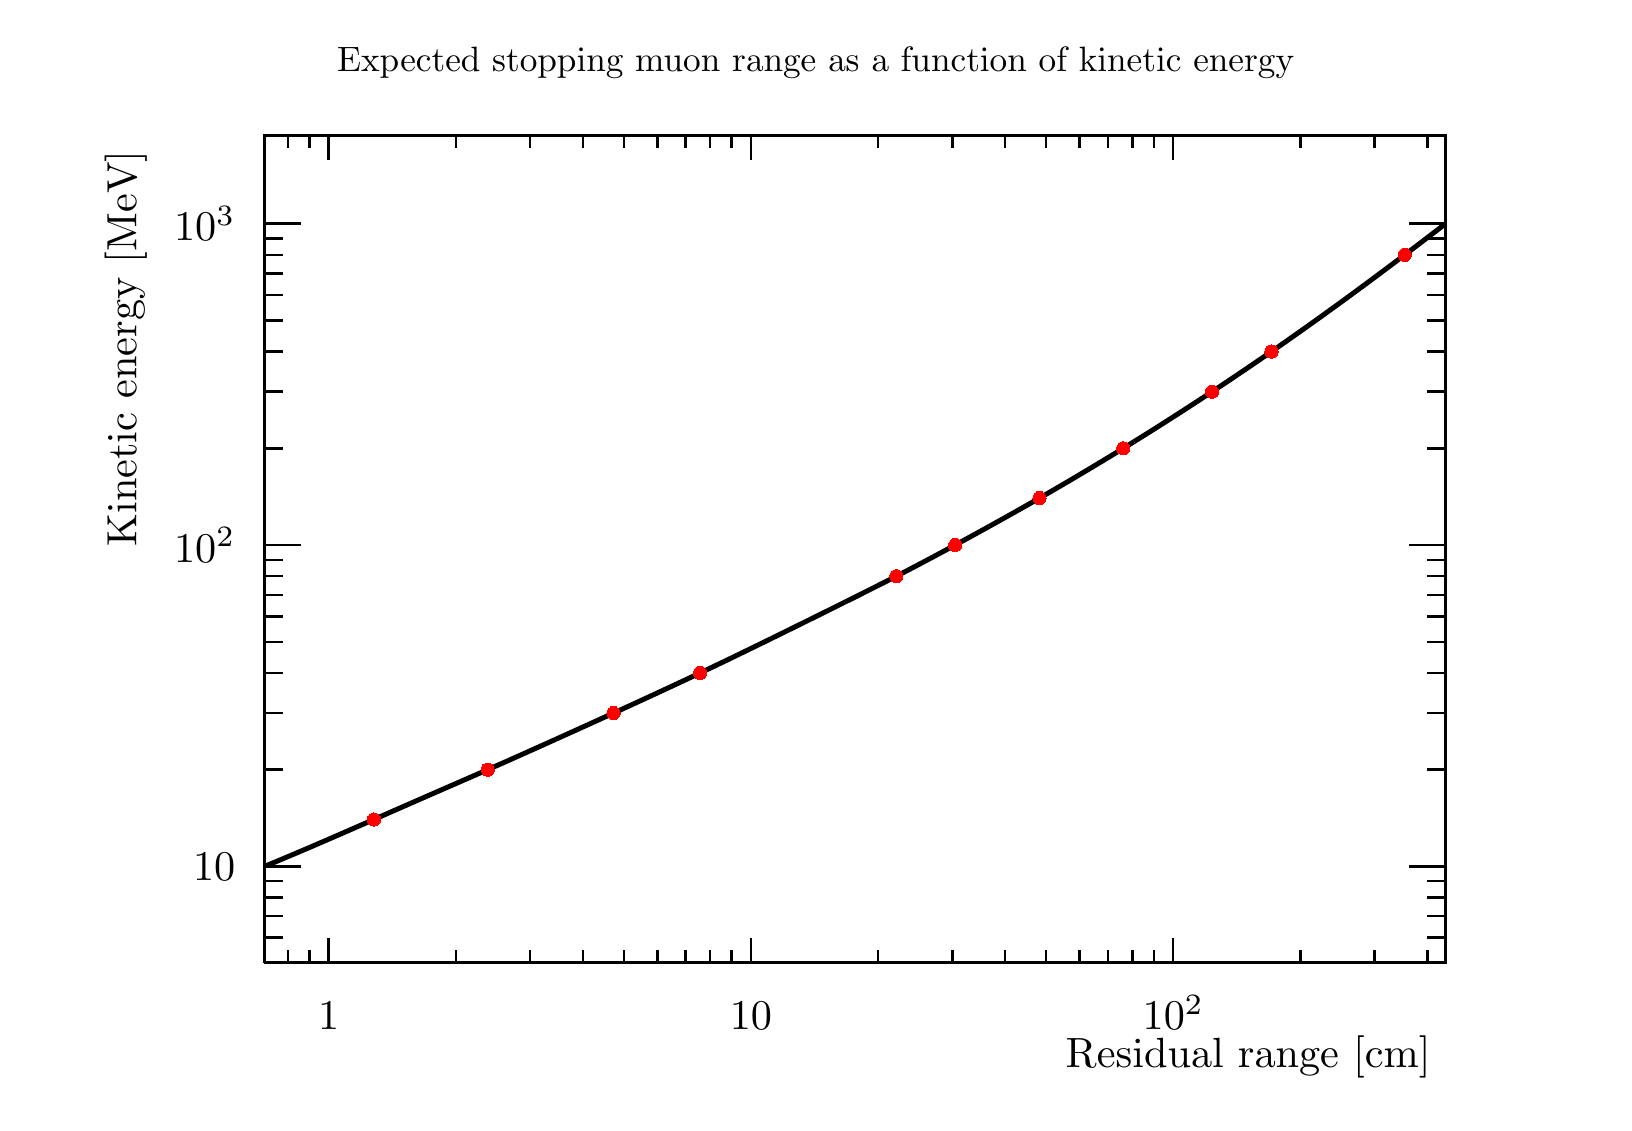
\begin{tikzpicture}
\pgfdeclareplotmark{cross} {
\pgfpathmoveto{\pgfpoint{-0.3\pgfplotmarksize}{\pgfplotmarksize}}
\pgfpathlineto{\pgfpoint{+0.3\pgfplotmarksize}{\pgfplotmarksize}}
\pgfpathlineto{\pgfpoint{+0.3\pgfplotmarksize}{0.3\pgfplotmarksize}}
\pgfpathlineto{\pgfpoint{+1\pgfplotmarksize}{0.3\pgfplotmarksize}}
\pgfpathlineto{\pgfpoint{+1\pgfplotmarksize}{-0.3\pgfplotmarksize}}
\pgfpathlineto{\pgfpoint{+0.3\pgfplotmarksize}{-0.3\pgfplotmarksize}}
\pgfpathlineto{\pgfpoint{+0.3\pgfplotmarksize}{-1.\pgfplotmarksize}}
\pgfpathlineto{\pgfpoint{-0.3\pgfplotmarksize}{-1.\pgfplotmarksize}}
\pgfpathlineto{\pgfpoint{-0.3\pgfplotmarksize}{-0.3\pgfplotmarksize}}
\pgfpathlineto{\pgfpoint{-1.\pgfplotmarksize}{-0.3\pgfplotmarksize}}
\pgfpathlineto{\pgfpoint{-1.\pgfplotmarksize}{0.3\pgfplotmarksize}}
\pgfpathlineto{\pgfpoint{-0.3\pgfplotmarksize}{0.3\pgfplotmarksize}}
\pgfpathclose
\pgfusepathqstroke
}
\pgfdeclareplotmark{cross*} {
\pgfpathmoveto{\pgfpoint{-0.3\pgfplotmarksize}{\pgfplotmarksize}}
\pgfpathlineto{\pgfpoint{+0.3\pgfplotmarksize}{\pgfplotmarksize}}
\pgfpathlineto{\pgfpoint{+0.3\pgfplotmarksize}{0.3\pgfplotmarksize}}
\pgfpathlineto{\pgfpoint{+1\pgfplotmarksize}{0.3\pgfplotmarksize}}
\pgfpathlineto{\pgfpoint{+1\pgfplotmarksize}{-0.3\pgfplotmarksize}}
\pgfpathlineto{\pgfpoint{+0.3\pgfplotmarksize}{-0.3\pgfplotmarksize}}
\pgfpathlineto{\pgfpoint{+0.3\pgfplotmarksize}{-1.\pgfplotmarksize}}
\pgfpathlineto{\pgfpoint{-0.3\pgfplotmarksize}{-1.\pgfplotmarksize}}
\pgfpathlineto{\pgfpoint{-0.3\pgfplotmarksize}{-0.3\pgfplotmarksize}}
\pgfpathlineto{\pgfpoint{-1.\pgfplotmarksize}{-0.3\pgfplotmarksize}}
\pgfpathlineto{\pgfpoint{-1.\pgfplotmarksize}{0.3\pgfplotmarksize}}
\pgfpathlineto{\pgfpoint{-0.3\pgfplotmarksize}{0.3\pgfplotmarksize}}
\pgfpathclose
\pgfusepathqfillstroke
}
\pgfdeclareplotmark{newstar} {
\pgfpathmoveto{\pgfqpoint{0pt}{\pgfplotmarksize}}
\pgfpathlineto{\pgfqpointpolar{44}{0.5\pgfplotmarksize}}
\pgfpathlineto{\pgfqpointpolar{18}{\pgfplotmarksize}}
\pgfpathlineto{\pgfqpointpolar{-20}{0.5\pgfplotmarksize}}
\pgfpathlineto{\pgfqpointpolar{-54}{\pgfplotmarksize}}
\pgfpathlineto{\pgfqpointpolar{-90}{0.5\pgfplotmarksize}}
\pgfpathlineto{\pgfqpointpolar{234}{\pgfplotmarksize}}
\pgfpathlineto{\pgfqpointpolar{198}{0.5\pgfplotmarksize}}
\pgfpathlineto{\pgfqpointpolar{162}{\pgfplotmarksize}}
\pgfpathlineto{\pgfqpointpolar{134}{0.5\pgfplotmarksize}}
\pgfpathclose
\pgfusepathqstroke
}
\pgfdeclareplotmark{newstar*} {
\pgfpathmoveto{\pgfqpoint{0pt}{\pgfplotmarksize}}
\pgfpathlineto{\pgfqpointpolar{44}{0.5\pgfplotmarksize}}
\pgfpathlineto{\pgfqpointpolar{18}{\pgfplotmarksize}}
\pgfpathlineto{\pgfqpointpolar{-20}{0.5\pgfplotmarksize}}
\pgfpathlineto{\pgfqpointpolar{-54}{\pgfplotmarksize}}
\pgfpathlineto{\pgfqpointpolar{-90}{0.5\pgfplotmarksize}}
\pgfpathlineto{\pgfqpointpolar{234}{\pgfplotmarksize}}
\pgfpathlineto{\pgfqpointpolar{198}{0.5\pgfplotmarksize}}
\pgfpathlineto{\pgfqpointpolar{162}{\pgfplotmarksize}}
\pgfpathlineto{\pgfqpointpolar{134}{0.5\pgfplotmarksize}}
\pgfpathclose
\pgfusepathqfillstroke
}
\definecolor{c}{rgb}{1,1,1};
\draw [color=c, fill=c] (0,0) rectangle (20,13.639);
\draw [color=c, fill=c] (3,1.77307) rectangle (18,12.2751);
\definecolor{c}{rgb}{0,0,0};
\draw [c,line width=0.9] (3,1.77307) -- (3,12.2751) -- (18,12.2751) -- (18,1.77307) -- (3,1.77307);
\definecolor{c}{rgb}{1,1,1};
\draw [color=c, fill=c] (0,0) rectangle (20,13.639);
\draw [color=c, fill=c] (3,1.77307) rectangle (18,12.2751);
\definecolor{c}{rgb}{0,0,0};
\draw [c,line width=0.9] (3,1.77307) -- (3,12.2751) -- (18,12.2751) -- (18,1.77307) -- (3,1.77307);
\draw [c,line width=1.8] (3.01883,3.00168) -- (3.05633,3.01716) -- (3.09383,3.03268) -- (3.13133,3.04826) -- (3.16883,3.06388) -- (3.20633,3.07955) -- (3.24383,3.09526) -- (3.28133,3.11102) -- (3.31883,3.12682) -- (3.35633,3.14266) --
 (3.39383,3.15854) -- (3.43133,3.17446) -- (3.46883,3.19042) -- (3.50633,3.20641) -- (3.54383,3.22244) -- (3.58133,3.2385) -- (3.61883,3.25459) -- (3.65633,3.27071) -- (3.69383,3.28686) -- (3.73133,3.30304) -- (3.76883,3.31925) -- (3.80633,3.33548)
 -- (3.84383,3.35173) -- (3.88133,3.36801) -- (3.91883,3.38431) -- (3.95633,3.40063) -- (3.99383,3.41696) -- (4.03133,3.43332) -- (4.06883,3.44968) -- (4.10633,3.46607) -- (4.14383,3.48246) -- (4.18133,3.49887) -- (4.21883,3.51529) --
 (4.25633,3.53172) -- (4.29383,3.54816) -- (4.33133,3.5646) -- (4.36883,3.58105) -- (4.40633,3.59751) -- (4.44383,3.61397) -- (4.48133,3.63043) -- (4.51883,3.64689) -- (4.55633,3.66335) -- (4.59383,3.67982) -- (4.63133,3.69628) -- (4.66883,3.71274)
 -- (4.70633,3.72919) -- (4.74383,3.74565) -- (4.78133,3.7621) -- (4.81883,3.77854) -- (4.85633,3.79498);
\draw [c,line width=1.8] (4.85633,3.79498) -- (4.89383,3.81141) -- (4.93133,3.82784) -- (4.96883,3.84426) -- (5.00633,3.86067) -- (5.04383,3.87707) -- (5.08133,3.89347) -- (5.11883,3.90986) -- (5.15633,3.92625) -- (5.19383,3.94262) -- (5.23133,3.959)
 -- (5.26883,3.97536) -- (5.30633,3.99172) -- (5.34383,4.00808) -- (5.38133,4.02444) -- (5.41883,4.04079) -- (5.45633,4.05714) -- (5.49383,4.0735) -- (5.53133,4.08985) -- (5.56883,4.10621) -- (5.60633,4.12258) -- (5.64383,4.13896) --
 (5.68133,4.15535) -- (5.71883,4.17176) -- (5.75633,4.18818) -- (5.79383,4.20463) -- (5.83133,4.2211) -- (5.86883,4.2376) -- (5.90633,4.25413) -- (5.94383,4.27069) -- (5.98133,4.28727) -- (6.01883,4.30388) -- (6.05633,4.32052) -- (6.09383,4.33717) --
 (6.13133,4.35385) -- (6.16883,4.37055) -- (6.20633,4.38728) -- (6.24383,4.40402) -- (6.28133,4.42077) -- (6.31883,4.43755) -- (6.35633,4.45434) -- (6.39383,4.47115) -- (6.43133,4.48797) -- (6.46883,4.50481) -- (6.50633,4.52165) -- (6.54383,4.53851)
 -- (6.58133,4.55538) -- (6.61883,4.57227) -- (6.65633,4.58916) -- (6.69383,4.60606);
\draw [c,line width=1.8] (6.69383,4.60606) -- (6.73133,4.62297) -- (6.76883,4.63989) -- (6.80633,4.65682) -- (6.84383,4.67375) -- (6.88133,4.6907) -- (6.91883,4.70765) -- (6.95633,4.72461) -- (6.99383,4.74157) -- (7.03133,4.75855) --
 (7.06883,4.77553) -- (7.10633,4.79252) -- (7.14383,4.80952) -- (7.18133,4.82653) -- (7.21883,4.84356) -- (7.25633,4.86059) -- (7.29383,4.87764) -- (7.33133,4.89469) -- (7.36883,4.91177) -- (7.40633,4.92886) -- (7.44383,4.94597) -- (7.48133,4.9631)
 -- (7.51883,4.98025) -- (7.55633,4.99741) -- (7.59383,5.0146) -- (7.63133,5.0318) -- (7.66883,5.04902) -- (7.70633,5.06626) -- (7.74383,5.08351) -- (7.78133,5.10078) -- (7.81883,5.11806) -- (7.85633,5.13537) -- (7.89383,5.15268) -- (7.93133,5.17002)
 -- (7.96883,5.18737) -- (8.00633,5.20474) -- (8.04383,5.22213) -- (8.08133,5.23954) -- (8.11883,5.25696) -- (8.15633,5.27441) -- (8.19383,5.29188) -- (8.23133,5.30936) -- (8.26883,5.32688) -- (8.30633,5.34442) -- (8.34383,5.36198) --
 (8.38133,5.37957) -- (8.41883,5.3972) -- (8.45633,5.41485) -- (8.49383,5.43254) -- (8.53133,5.45027);
\draw [c,line width=1.8] (8.53133,5.45027) -- (8.56883,5.46804) -- (8.60633,5.48585) -- (8.64383,5.50369) -- (8.68133,5.52157) -- (8.71883,5.53949) -- (8.75633,5.55744) -- (8.79383,5.57543) -- (8.83133,5.59345) -- (8.86883,5.6115) --
 (8.90633,5.62958) -- (8.94383,5.64769) -- (8.98133,5.66582) -- (9.01883,5.68399) -- (9.05633,5.70218) -- (9.09383,5.72039) -- (9.13133,5.73863) -- (9.16883,5.75689) -- (9.20633,5.77517) -- (9.24383,5.79348) -- (9.28133,5.8118) -- (9.31883,5.83014)
 -- (9.35633,5.8485) -- (9.39383,5.86688) -- (9.43133,5.88527) -- (9.46883,5.90368) -- (9.50633,5.9221) -- (9.54383,5.94054) -- (9.58133,5.95899) -- (9.61883,5.97745) -- (9.65633,5.99593) -- (9.69383,6.01441) -- (9.73133,6.03291) -- (9.76883,6.05142)
 -- (9.80633,6.06994) -- (9.84383,6.08846) -- (9.88133,6.107) -- (9.91883,6.12555) -- (9.95633,6.1441) -- (9.99383,6.16267) -- (10.0313,6.18124) -- (10.0688,6.19983) -- (10.1063,6.21842) -- (10.1438,6.23702) -- (10.1813,6.25564) -- (10.2188,6.27426)
 -- (10.2563,6.2929) -- (10.2938,6.31154) -- (10.3313,6.3302) -- (10.3688,6.34888);
\draw [c,line width=1.8] (10.3688,6.34888) -- (10.4063,6.36757) -- (10.4438,6.38628) -- (10.4813,6.405) -- (10.5188,6.42374) -- (10.5563,6.44251) -- (10.5938,6.4613) -- (10.6313,6.48011) -- (10.6688,6.49895) -- (10.7063,6.51782) -- (10.7438,6.53673)
 -- (10.7813,6.55567) -- (10.8188,6.57464) -- (10.8563,6.59366) -- (10.8938,6.61273) -- (10.9313,6.63185) -- (10.9688,6.65102) -- (11.0063,6.67025) -- (11.0438,6.68954) -- (11.0813,6.7089) -- (11.1188,6.72832) -- (11.1563,6.7478) -- (11.1938,6.76735)
 -- (11.2313,6.78695) -- (11.2688,6.80662) -- (11.3063,6.82634) -- (11.3438,6.84611) -- (11.3813,6.86594) -- (11.4188,6.88583) -- (11.4563,6.90577) -- (11.4938,6.92575) -- (11.5313,6.94579) -- (11.5688,6.96587) -- (11.6063,6.986) -- (11.6438,7.00617)
 -- (11.6813,7.02639) -- (11.7188,7.04665) -- (11.7563,7.06694) -- (11.7938,7.08728) -- (11.8313,7.10765) -- (11.8688,7.12806) -- (11.9063,7.14851) -- (11.9438,7.16899) -- (11.9813,7.18951) -- (12.0188,7.21006) -- (12.0563,7.23065) --
 (12.0938,7.25128) -- (12.1313,7.27194) -- (12.1688,7.29264) -- (12.2063,7.31338);
\draw [c,line width=1.8] (12.2063,7.31338) -- (12.2438,7.33416) -- (12.2813,7.35497) -- (12.3188,7.37582) -- (12.3563,7.39671) -- (12.3938,7.41764) -- (12.4313,7.4386) -- (12.4688,7.45961) -- (12.5063,7.48066) -- (12.5438,7.50176) --
 (12.5813,7.52289) -- (12.6188,7.54408) -- (12.6563,7.5653) -- (12.6938,7.58658) -- (12.7313,7.60791) -- (12.7688,7.62928) -- (12.8063,7.65071) -- (12.8438,7.67219) -- (12.8813,7.69374) -- (12.9188,7.71533) -- (12.9563,7.73698) -- (12.9938,7.75869)
 -- (13.0313,7.78046) -- (13.0688,7.80227) -- (13.1063,7.82415) -- (13.1438,7.84607) -- (13.1813,7.86806) -- (13.2188,7.89009) -- (13.2563,7.91218) -- (13.2938,7.93432) -- (13.3313,7.95652) -- (13.3688,7.97877) -- (13.4063,8.00107) --
 (13.4438,8.02342) -- (13.4813,8.04583) -- (13.5188,8.06829) -- (13.5563,8.09081) -- (13.5938,8.11338) -- (13.6313,8.136) -- (13.6688,8.15868) -- (13.7063,8.18141) -- (13.7438,8.20419) -- (13.7813,8.22704) -- (13.8188,8.24993) -- (13.8563,8.27289) --
 (13.8938,8.2959) -- (13.9313,8.31897) -- (13.9688,8.3421) -- (14.0063,8.36528) -- (14.0438,8.38852);
\draw [c,line width=1.8] (14.0438,8.38852) -- (14.0813,8.41182) -- (14.1188,8.43518) -- (14.1563,8.45859) -- (14.1938,8.48206) -- (14.2313,8.50558) -- (14.2688,8.52916) -- (14.3063,8.55279) -- (14.3438,8.57648) -- (14.3813,8.60023) --
 (14.4188,8.62403) -- (14.4563,8.64788) -- (14.4938,8.67179) -- (14.5313,8.69575) -- (14.5688,8.71977) -- (14.6063,8.74385) -- (14.6438,8.76797) -- (14.6813,8.79216) -- (14.7188,8.8164) -- (14.7563,8.84069) -- (14.7938,8.86504) -- (14.8313,8.88945)
 -- (14.8688,8.91391) -- (14.9063,8.93843) -- (14.9438,8.96301) -- (14.9813,8.98765) -- (15.0188,9.01234) -- (15.0563,9.03709) -- (15.0938,9.0619) -- (15.1313,9.08677) -- (15.1688,9.1117) -- (15.2063,9.13669) -- (15.2438,9.16174) -- (15.2813,9.18684)
 -- (15.3188,9.21201) -- (15.3563,9.23723) -- (15.3938,9.26252) -- (15.4313,9.28786) -- (15.4688,9.31326) -- (15.5063,9.33872) -- (15.5438,9.36424) -- (15.5813,9.38982) -- (15.6188,9.41546) -- (15.6563,9.44116) -- (15.6938,9.46692) --
 (15.7313,9.49275) -- (15.7688,9.51863) -- (15.8063,9.54458) -- (15.8438,9.57059) -- (15.8813,9.59666);
\draw [c,line width=1.8] (15.8813,9.59666) -- (15.9188,9.62279) -- (15.9563,9.64898) -- (15.9938,9.67524) -- (16.0313,9.70155) -- (16.0688,9.72792) -- (16.1063,9.75436) -- (16.1438,9.78085) -- (16.1813,9.8074) -- (16.2188,9.834) -- (16.2563,9.86067)
 -- (16.2938,9.88739) -- (16.3313,9.91416) -- (16.3688,9.941) -- (16.4063,9.96789) -- (16.4438,9.99483) -- (16.4813,10.0218) -- (16.5188,10.0489) -- (16.5563,10.076) -- (16.5938,10.1031) -- (16.6313,10.1304) -- (16.6688,10.1576) -- (16.7063,10.1849)
 -- (16.7438,10.2123) -- (16.7813,10.2397) -- (16.8188,10.2672) -- (16.8563,10.2947) -- (16.8938,10.3223) -- (16.9313,10.3499) -- (16.9688,10.3776) -- (17.0063,10.4053) -- (17.0438,10.4331) -- (17.0813,10.4609) -- (17.1188,10.4888) --
 (17.1563,10.5167) -- (17.1938,10.5447) -- (17.2313,10.5727) -- (17.2688,10.6008) -- (17.3063,10.6289) -- (17.3438,10.657) -- (17.3813,10.6852) -- (17.4188,10.7135) -- (17.4563,10.7418) -- (17.4938,10.7701) -- (17.5313,10.7985) -- (17.5688,10.8269)
 -- (17.6063,10.8554) -- (17.6438,10.8839) -- (17.6813,10.9124) -- (17.7188,10.941);
\draw [c,line width=1.8] (17.7188,10.941) -- (17.7563,10.9696) -- (17.7938,10.9983) -- (17.8313,11.027) -- (17.8688,11.0558) -- (17.9063,11.0846) -- (17.9438,11.1134) -- (17.9813,11.1423);
\draw [c,line width=0.9] (3,1.77307) -- (18,1.77307);
\draw [c,line width=0.9] (3.2965,1.9265) -- (3.2965,1.77307);
\draw [c,line width=0.9] (3.57082,1.9265) -- (3.57082,1.77307);
\draw [c,line width=0.9] (3.8162,2.07994) -- (3.8162,1.77307);
\draw [anchor=base] (3.8162,0.92063) node[scale=1.52731, color=c, rotate=0]{1};
\draw [c,line width=0.9] (5.43053,1.9265) -- (5.43053,1.77307);
\draw [c,line width=0.9] (6.37485,1.9265) -- (6.37485,1.77307);
\draw [c,line width=0.9] (7.04486,1.9265) -- (7.04486,1.77307);
\draw [c,line width=0.9] (7.56456,1.9265) -- (7.56456,1.77307);
\draw [c,line width=0.9] (7.98918,1.9265) -- (7.98918,1.77307);
\draw [c,line width=0.9] (8.34819,1.9265) -- (8.34819,1.77307);
\draw [c,line width=0.9] (8.65919,1.9265) -- (8.65919,1.77307);
\draw [c,line width=0.9] (8.9335,1.9265) -- (8.9335,1.77307);
\draw [c,line width=0.9] (9.17888,2.07994) -- (9.17888,1.77307);
\draw [anchor=base] (9.17888,0.92063) node[scale=1.52731, color=c, rotate=0]{10};
\draw [c,line width=0.9] (10.7932,1.9265) -- (10.7932,1.77307);
\draw [c,line width=0.9] (11.7375,1.9265) -- (11.7375,1.77307);
\draw [c,line width=0.9] (12.4075,1.9265) -- (12.4075,1.77307);
\draw [c,line width=0.9] (12.9272,1.9265) -- (12.9272,1.77307);
\draw [c,line width=0.9] (13.3519,1.9265) -- (13.3519,1.77307);
\draw [c,line width=0.9] (13.7109,1.9265) -- (13.7109,1.77307);
\draw [c,line width=0.9] (14.0219,1.9265) -- (14.0219,1.77307);
\draw [c,line width=0.9] (14.2962,1.9265) -- (14.2962,1.77307);
\draw [c,line width=0.9] (14.5416,2.07994) -- (14.5416,1.77307);
\draw [anchor=base] (14.5416,0.92063) node[scale=1.52731, color=c, rotate=0]{$10^{2}$};
\draw [c,line width=0.9] (16.1559,1.9265) -- (16.1559,1.77307);
\draw [c,line width=0.9] (17.1002,1.9265) -- (17.1002,1.77307);
\draw [c,line width=0.9] (17.7702,1.9265) -- (17.7702,1.77307);
\draw [anchor= east] (18,0.572837) node[scale=1.52731, color=c, rotate=0]{ Residual range [cm]};
\draw [c,line width=0.9] (3,12.2751) -- (18,12.2751);
\draw [c,line width=0.9] (3.2965,12.1216) -- (3.2965,12.2751);
\draw [c,line width=0.9] (3.57082,12.1216) -- (3.57082,12.2751);
\draw [c,line width=0.9] (3.8162,11.9682) -- (3.8162,12.2751);
\draw [c,line width=0.9] (5.43053,12.1216) -- (5.43053,12.2751);
\draw [c,line width=0.9] (6.37485,12.1216) -- (6.37485,12.2751);
\draw [c,line width=0.9] (7.04486,12.1216) -- (7.04486,12.2751);
\draw [c,line width=0.9] (7.56456,12.1216) -- (7.56456,12.2751);
\draw [c,line width=0.9] (7.98918,12.1216) -- (7.98918,12.2751);
\draw [c,line width=0.9] (8.34819,12.1216) -- (8.34819,12.2751);
\draw [c,line width=0.9] (8.65919,12.1216) -- (8.65919,12.2751);
\draw [c,line width=0.9] (8.9335,12.1216) -- (8.9335,12.2751);
\draw [c,line width=0.9] (9.17888,11.9682) -- (9.17888,12.2751);
\draw [c,line width=0.9] (10.7932,12.1216) -- (10.7932,12.2751);
\draw [c,line width=0.9] (11.7375,12.1216) -- (11.7375,12.2751);
\draw [c,line width=0.9] (12.4075,12.1216) -- (12.4075,12.2751);
\draw [c,line width=0.9] (12.9272,12.1216) -- (12.9272,12.2751);
\draw [c,line width=0.9] (13.3519,12.1216) -- (13.3519,12.2751);
\draw [c,line width=0.9] (13.7109,12.1216) -- (13.7109,12.2751);
\draw [c,line width=0.9] (14.0219,12.1216) -- (14.0219,12.2751);
\draw [c,line width=0.9] (14.2962,12.1216) -- (14.2962,12.2751);
\draw [c,line width=0.9] (14.5416,11.9682) -- (14.5416,12.2751);
\draw [c,line width=0.9] (16.1559,12.1216) -- (16.1559,12.2751);
\draw [c,line width=0.9] (17.1002,12.1216) -- (17.1002,12.2751);
\draw [c,line width=0.9] (17.7702,12.1216) -- (17.7702,12.2751);
\draw [c,line width=0.9] (3,1.77307) -- (3,12.2751);
\draw [c,line width=0.9] (3.231,2.08848) -- (3,2.08848);
\draw [c,line width=0.9] (3.231,2.36172) -- (3,2.36172);
\draw [c,line width=0.9] (3.231,2.5984) -- (3,2.5984);
\draw [c,line width=0.9] (3.231,2.80718) -- (3,2.80718);
\draw [c,line width=0.9] (3.462,2.99393) -- (3,2.99393);
\draw [anchor= east] (2.82,2.99393) node[scale=1.52731, color=c, rotate=0]{10};
\draw [c,line width=0.9] (3.231,4.22255) -- (3,4.22255);
\draw [c,line width=0.9] (3.231,4.94124) -- (3,4.94124);
\draw [c,line width=0.9] (3.231,5.45116) -- (3,5.45116);
\draw [c,line width=0.9] (3.231,5.84669) -- (3,5.84669);
\draw [c,line width=0.9] (3.231,6.16986) -- (3,6.16986);
\draw [c,line width=0.9] (3.231,6.44309) -- (3,6.44309);
\draw [c,line width=0.9] (3.231,6.67978) -- (3,6.67978);
\draw [c,line width=0.9] (3.231,6.88855) -- (3,6.88855);
\draw [c,line width=0.9] (3.462,7.07531) -- (3,7.07531);
\draw [anchor= east] (2.82,7.07531) node[scale=1.52731, color=c, rotate=0]{$10^{2}$};
\draw [c,line width=0.9] (3.231,8.30392) -- (3,8.30392);
\draw [c,line width=0.9] (3.231,9.02262) -- (3,9.02262);
\draw [c,line width=0.9] (3.231,9.53254) -- (3,9.53254);
\draw [c,line width=0.9] (3.231,9.92807) -- (3,9.92807);
\draw [c,line width=0.9] (3.231,10.2512) -- (3,10.2512);
\draw [c,line width=0.9] (3.231,10.5245) -- (3,10.5245);
\draw [c,line width=0.9] (3.231,10.7612) -- (3,10.7612);
\draw [c,line width=0.9] (3.231,10.9699) -- (3,10.9699);
\draw [c,line width=0.9] (3.462,11.1567) -- (3,11.1567);
\draw [anchor= east] (2.82,11.1567) node[scale=1.52731, color=c, rotate=0]{$10^{3}$};
\draw [anchor= east] (1.24,12.2751) node[scale=1.52731, color=c, rotate=90]{ Kinetic energy [MeV]};
\draw [c,line width=0.9] (18,1.77307) -- (18,12.2751);
\draw [c,line width=0.9] (17.769,2.08848) -- (18,2.08848);
\draw [c,line width=0.9] (17.769,2.36172) -- (18,2.36172);
\draw [c,line width=0.9] (17.769,2.5984) -- (18,2.5984);
\draw [c,line width=0.9] (17.769,2.80718) -- (18,2.80718);
\draw [c,line width=0.9] (17.538,2.99393) -- (18,2.99393);
\draw [c,line width=0.9] (17.769,4.22255) -- (18,4.22255);
\draw [c,line width=0.9] (17.769,4.94124) -- (18,4.94124);
\draw [c,line width=0.9] (17.769,5.45116) -- (18,5.45116);
\draw [c,line width=0.9] (17.769,5.84669) -- (18,5.84669);
\draw [c,line width=0.9] (17.769,6.16986) -- (18,6.16986);
\draw [c,line width=0.9] (17.769,6.44309) -- (18,6.44309);
\draw [c,line width=0.9] (17.769,6.67978) -- (18,6.67978);
\draw [c,line width=0.9] (17.769,6.88855) -- (18,6.88855);
\draw [c,line width=0.9] (17.538,7.07531) -- (18,7.07531);
\draw [c,line width=0.9] (17.769,8.30392) -- (18,8.30392);
\draw [c,line width=0.9] (17.769,9.02262) -- (18,9.02262);
\draw [c,line width=0.9] (17.769,9.53254) -- (18,9.53254);
\draw [c,line width=0.9] (17.769,9.92807) -- (18,9.92807);
\draw [c,line width=0.9] (17.769,10.2512) -- (18,10.2512);
\draw [c,line width=0.9] (17.769,10.5245) -- (18,10.5245);
\draw [c,line width=0.9] (17.769,10.7612) -- (18,10.7612);
\draw [c,line width=0.9] (17.769,10.9699) -- (18,10.9699);
\draw [c,line width=0.9] (17.538,11.1567) -- (18,11.1567);
\definecolor{c}{rgb}{1,0,0};
\foreach \P in {(4.38998,3.59034), (5.83462,4.22255), (7.43347,4.94124), (8.53322,5.45117), (11.0249,6.67978), (11.7718,7.07531), (12.843,7.67171), (13.9069,8.30392), (15.0344,9.02262), (15.7889,9.53254), (17.482,10.7612)}{\draw[mark
 options={color=c,fill=c},mark size=2.402402pt, line width=0.000000pt, mark=*] plot coordinates {\P};}
\definecolor{c}{rgb}{1,1,1};
\draw [color=c, fill=c] (2,12.8206) rectangle (18,13.5708);
\definecolor{c}{rgb}{0,0,0};
\draw (10,13.1957) node[scale=1.27276, color=c, rotate=0]{Expected stopping muon range as a function of kinetic energy};
\end{tikzpicture}

	\end{adjustbox}
	\caption[Muon range in liquid argon as a function of kinetic energy]{Muon range in liquid argon under the continuous slowing down approximation (CSDA) as a function of kinetic energy. The red points are taken from~\cite{muonCSDA}. The black line is a cubic spline drawn through the points.}
	\label{fig:keVsRange}
\end{figure}

%% Track selection
From \citefig{fig:muonEDep} left and right, one can see that, aside from the last 40 or \SI{50}{\cm} of the track, muons will have uniform energy deposition in liquid argon.
Therefore, any track selection used for detector calibration should avoid using the ends of muon tracks.
However, excluding the last \SI{50}{\cm} of all muon tracks regardless of if they stop in the detector or not would result in a significant volume of the detector which could not be effectively calibrated by this method.
Therefore, it is decided to instead select all those cosmic ray tracks which exit the detector and assume that they are not close to stopping.
Specifically, those tracks that cross the cathode and at least one of the anodes are selected.

Requiring that tracks cross the cathode and an anode has two outcomes.
Firstly, it ensures that all the selected tracks have lengths equal to at least the drift distance and excludes short tracks that may be more easily mis-reconstructed.

Secondly, it allows the tracks to be given a definite time at which they entered the TPC.
As mentioned in \citesec{sec:dune:fd:lartpc}, TPCs such as ProtoDUNE-SP produce multiple 2-dimensional images which can be combined via reconstruction algorithms~\cite{pandora} to form 3-dimensional reconstructed tracks.
Typically, for neutrino induced events in LAr TPCs a definite drift coordinate can be reconstructed using timing information from the neutrino beam.

However for external particles such as cosmic rays, which are impinging on the detector continuously, this beam timing information is obviously not available.
Instead, reconstruction techniques must be utilised.

Specifically, the Pandora software package~\cite{pandora} looks at tracks in the two TPCs, separated by the central cathode.
If two 3-dimensional clusters in neighbouring drift volumes have similar direction vectors and an equal and opposite shift in the drift direction from the cathode, they can be stitched across the cathode to form one larger track.
This track will therefore have a definite time at which it crossed the cathode, often termed a $t_{0}$.
In turn, this allows definite drift coordinates to be reconstructed for all points in the track.


%% Angular cuts explanation

\section{Impact on far detector measurements}
\label{sec:pdune_calibration:fd}